\documentclass[10pt]{article}
\usepackage[polish]{babel}
\usepackage[utf8]{inputenc}
\usepackage[T1]{fontenc}
\usepackage{amsmath}
\usepackage{amsfonts}
\usepackage{amssymb}
\usepackage[version=4]{mhchem}
\usepackage{stmaryrd}
\usepackage{graphicx}
\usepackage[export]{adjustbox}
\graphicspath{ {./images/} }

\begin{document}
\section*{CENTRALNA \\
 KOMISJA \\
 EGZAMINACYJNA}
\begin{center}
\begin{tabular}{|l|l|}
\hline
Rodzaj dokumentu: & \begin{tabular}{l}
ZaSady Oceniania rozwiązań \\
zadań \\
\end{tabular} \\
\hline
Egzamin: & Egzamin maturalny \\
\hline
Przedmiot: & Matematyka \\
\hline
Poziom: & Poziom rozSzerzony \\
\hline
Formy arkusza: & \begin{tabular}{l}
MMA-R1\_1P-202, MMA-R1\_2P-202, \\
MMA-R1\_3P-202, MMA-R1\_4P-202, \\
MMA-R1\_5P-202, MMA-R1\_6P-202, \\
MMA-R1\_7P-202, MMA-R1\_QP-202 \\
\end{tabular} \\
\hline
Termin egzaminu: & Termin główny - czerwiec 2020 r. \\
\hline
\begin{tabular}{l}
Data publikacji \\
dokumentu: \\
\end{tabular} & 3 sierpnia 2020 r. \\
\hline
\end{tabular}
\end{center}

\section*{Zadania zamknięte}
W zadaniach 1.-4. przyznaje się punkt za wskazanie poprawnej odpowiedzi.

\section*{Zadanie 1. (0-1)}
\begin{center}
\begin{tabular}{|l|l|c|}
\hline
\multicolumn{1}{|c|}{Wymaganie ogólne} & \multicolumn{1}{c|}{Wymaganie szczegółowe} & Poprawna odpowiedź \\
\hline
\begin{tabular}{l}
II. Wykorzystanie \\
i interpretowanie \\
reprezentacji. \\
\end{tabular} & \begin{tabular}{l}
3. Równania i nierówności. Zdający \\
stosuje twierdzenie o reszcie \\
z dzielenia wielomianu przez dwumian \\
x-a (R3.4). \\
\end{tabular} & B \\
\hline
\end{tabular}
\end{center}

Zadanie 2. (0-1)

\begin{center}
\begin{tabular}{|l|l|c|}
\hline
\multicolumn{1}{|c|}{Wymaganie ogólne} & \multicolumn{1}{c|}{Wymaganie szczegółowe} & Poprawna odpowiedź \\
\hline
\begin{tabular}{l}
II. Wykorzystanie \\
i interpretowanie \\
reprezentacji. \\
\end{tabular} & \begin{tabular}{l}
5. Ciągi. Zdający oblicza granice \\
ciągów, korzystając z granic ciągów \\
typu $\frac{1}{n}, \frac{1}{n^{2}}$ oraz z twierdzeń \\
o działaniach na granicach ciągów \\
(R5.2). \\
\end{tabular} &  \\
\hline
\end{tabular}
\end{center}

\section*{Zadanie 3. (0-1)}
\begin{center}
\begin{tabular}{|l|l|c|}
\hline
\multicolumn{1}{|c|}{Wymaganie ogólne} & \multicolumn{1}{c|}{Wymaganie szczegółowe} & Poprawna odpowiedź \\
\hline
\begin{tabular}{l}
III. Modelowanie \\
matematyczne \\
\end{tabular} & \begin{tabular}{l}
10. Elementy statystyki opisowej. \\
Teoria prawdopodobieństwa \\
i kombinatoryka. Zdający \\
wykorzystuje wzory na liczbe \\
permutacji, kombinacji, wariacji \\
i wariacji z powtórzenia mi do \\
zliczania obiektów w bardziej \\
złożonych sytuacjach \\
kombinatorycznych (R10.1). \\
\end{tabular} & A \\
\hline
\end{tabular}
\end{center}

\section*{Zadanie 4. (0-1)}
\begin{center}
\begin{tabular}{|l|l|c|}
\hline
\multicolumn{1}{|c|}{Wymaganie ogólne} & \multicolumn{1}{c|}{Wymaganie szczegółowe} & Poprawna odpowiedź \\
\hline
\begin{tabular}{l}
II. Wykorzystanie \\
i interpretowanie \\
reprezentacji. \\
\end{tabular} & \begin{tabular}{l}
2. Wyrażenia algebraiczne. Zdajácy \\
używa wzorów skróconego mnożenia \\
$(a \pm b)^{2}$ oraz $a^{2}-b^{2}$ (2.1). Zdający \\
używa wzorów skróconego mnożenia \\
$(a \pm b)^{3}$ oraz $a^{3} \pm b^{3}$ (R2.1). \\
\end{tabular} &  \\
\hline
\end{tabular}
\end{center}

\section*{Zadanie 5. (0-2)}
\begin{center}
\begin{tabular}{|l|l|l|l|l|}
\hline
\multicolumn{1}{|c|}{Wymagania ogólne} & \multicolumn{1}{|c|}{Wymagania szczegółowe} & \multicolumn{2}{|c|}{Poprawna odpowiedź} &  \\
\hline
\begin{tabular}{l}
IV. Użycie i tworzenie \\
strategii. \\
\end{tabular} & \begin{tabular}{l}
7. Planimetria. Zdający znajduje \\
związki miarowe w figurach płaskich \\
z zastosowaniem twierdzenia sinusów \\
i twierdzenia cosinusów (R7.5). \\
\end{tabular} & 9 & 5 & 5 \\
\hline
\end{tabular}
\end{center}

\section*{Zasady oceniania}
2 pkt - poprawna odpowiedź.\\
0 pkt - odpowiedź niepełna lub niepoprawna albo brak odpowiedzi.

Uwaga: Akceptowane są wszystkie rozwiązania merytorycznie poprawne i spełniające warunki zadania.

\section*{Zadanie 6. (0-3)}
\begin{center}
\begin{tabular}{|l|l|}
\hline
\multicolumn{1}{|c|}{Wymagania ogólne} & \multicolumn{1}{c|}{Wymagania szczegółowe} \\
\hline
IV. Użycie i tworzenie strategii. & \begin{tabular}{l}
1. Liczby rzeczywiste. Zdający wykorzystuje pojęcie \\
wartości bez względnej i jej interpretację \\
geometryczna (R1.1). \\
4. Funkcje. Zdający szkicuje wykres funkcji \\
określonej w różnych przedziałach różnymi wzorami; \\
odczytuje własności takiej funkcji z wykresu (R4.4). \\
\end{tabular} \\
\hline
\end{tabular}
\end{center}

\section*{Zasady oceniania I sposobu rozwiązania}
\section*{Rozwiązanie, w którym postęp jest wprawdzie niewielki, ale konieczny na drodze do pełnego rozwiązania zadania \\
 .1p.}
Zdający naszkicuje wykres funkcji $f$ określonej wzorem:

\begin{itemize}
  \item $f(x)=|x-5|$\\
albo
  \item $f(x)=|x-5|+4$\\
i na tym zakończy lub dalej popełni błędy.\\
Pokonanie zasadniczych trudności zadania 2p.
\end{itemize}

Zdający zapisze układ nierówności

\begin{itemize}
  \item $0<(a-1)^{2}-4<5$ oraz rozwiąże poprawnie jedną z nierówności tego układu\\
albo
  \item $4<(a-1)^{2}<9$ oraz rozwiąże poprawnie jedną z nierówności tego układu\\
i na tym zakończy lub dalej popełni błędy.\\
Rozwiązanie pełne 3p.
\end{itemize}

Zdający rozwiąże układ nierówności i zapisze, że $a \in(-2,-1) \cup(3,4)$.

\section*{Zasady oceniania II sposobu rozwiązania}
\section*{Rozwiązanie, w którym postęp jest wprawdzie niewielki, ale konieczny na drodze do pełnego rozwiązania zadania $1 p$.}
Zdający zapisze, że podane równanie ma dwa rozwiązania dodatnie, gdy spełniona jest nierówność

$$
0<|x-5|<5
$$

i na tym zakończy lub dalej popełni błędy.\\
Pokonanie zasadniczych trudności zadania 2p.

Zdający zapisze układ nierówności $0<(a-1)^{2}-4<5$ oraz rozwiąże poprawnie jedną z dwóch nierówności tego układu i na tym zakończy lub dalej popełni błędy.

Rozwiązanie pełne 3p.\\
Zdający rozwiąże układ nierówności i zapisze, że $a \in(-2,-1) \cup(3,4)$.

\section*{Zasady oceniania III sposobu rozwiązania}
Rozwiązanie, w którym postęp jest wprawdzie niewielki, ale konieczny na drodze do pełnego rozwiązania zadania\\
.1p.\\
Zdający:

\begin{itemize}
  \item zapisze, że podane równanie ma więcej niż jedno rozwiązanie wtedy, gdy spełniona jest nierówność
\end{itemize}

$$
(a-1)^{2}-4>0
$$

albo

\begin{itemize}
  \item zapisze podane równanie w postaci alternatywy równań
\end{itemize}

$$
x-5=(a-1)^{2}-4 \quad \text { lub } \quad x-5=-(a-1)^{2}+4
$$

i na tym zakończy lub dalej popełni błędy.\\
Pokonanie zasadniczych trudności zadania 2p.\\
Zdający:

\begin{itemize}
  \item zapisze, że podane równanie ma więcej niż jedno rozwiązanie wtedy, gdy spełniona jest nierówność
\end{itemize}

$$
(a-1)^{2}-4>0
$$

i

\begin{itemize}
  \item zapisze podane równanie w postaci alternatywy równań
\end{itemize}

$$
x-5=(a-1)^{2}-4 \text { lub } x-5=-(a-1)^{2}+4
$$

i

\begin{itemize}
  \item rozwiąże poprawnie przynajmniej jedną z trzech nierówności:
\end{itemize}

$$
(a-1)^{2}-4>0,(a-1)^{2}+1>0,9-(a-1)^{2}>0
$$

i na tym zakończy lub dalej popełni błędy.\\
Rozwiązanie pełne 3p.\\
Zdający zapisze, że $a \in(-2,-1) \cup(3,4)$.

\section*{Zasady oceniania IV sposobu rozwiązania}
\section*{Rozwiązanie, w którym postęp jest wprawdzie niewielki, ale konieczny na drodze do pełnego rozwiązania zadania \\
 $1 p$. \\
 Zdający}
\begin{itemize}
  \item zapisze warunek istnienia rozwiązań rzeczywistych równania $|x-5|=(a-1)^{2}-4$ :
\end{itemize}

$$
(a-1)^{2}-4 \geq 0
$$

albo

\begin{itemize}
  \item zdający zapisze układ nierówności:
\end{itemize}

$$
(-10)^{2}-4\left(25-\left((a-1)^{2}-4\right)^{2}\right)>0 \quad \text { i } \frac{-(-10)}{1}>0 \quad \text { i } 25-\left((a-1)^{2}-4\right)^{2}>0
$$

i na tym zakończy lub dalej popełni błędy.\\
Pokonanie zasadniczych trudności zadania 2p.\\
Zdający zapisze układ nierówności\\
$(a-1)^{2}-4 \geq 0$ i $(-10)^{2}-4\left(25-\left((a-1)^{2}-4\right)^{2}\right)>0 \quad$ i $\quad \frac{-(-10)}{1}>0 \quad$ i $25-\left((a-1)^{2}-4\right)^{2}>0$\\
i poprawnie rozwiąże drugą lub czwartą z nich i na tym zakończy lub dalej popełni błędy.

\section*{Rozwiązanie pełne}
3p.\\
Zdający rozwiąże układ nierówności i zapisze, że $a \in(-2,-1) \cup(3,4)$.

\section*{Zasady oceniania V sposobu rozwiązania}
\section*{Rozwiązanie, w którym postęp jest wprawdzie niewielki, ale konieczny na drodze do pełnego rozwiązania zadania}
Zdający zastosuje definicję wartości bezwzględnej i zapisze równanie w każdym z dwóch przypadków:\\
gdy $x-5 \geq 0$, to $x-5=(a-1)^{2}-4$,\\
gdy $x-5<0$, to $5-x=(a-1)^{2}-4$\\
i na tym zakończy lub dalej popełni błędy.

\section*{Pokonanie zasadniczych trudności zadania}
Zdający zapisze warunki na to, żeby rozwiązaniem równania była liczba dodatnia w każdym z dwóch rozpatrywanych przypadków i wyznaczy wszystkie wartości parametru a, dla których rozwiązaniem równania jest liczba dodatnia w jednym z tych przypadków:

\begin{itemize}
  \item gdy $x-5 \geq 0$, to $(a-1)^{2}+1>0$ i $(a-1)^{2}+1 \geq 5$, skąd $a \in(-\infty,-1\rangle \cup\langle 3,+\infty)$\\
albo
  \item gdy $x-5<0$, to $9-(a-1)^{2}>0$ i $9-(a-1)^{2}<5$, skąd $a \in(-2,-1) \cup(3,4)$\\
i na tym zakończy lub dalej popełni błędy.\\
Rozwiązanie pełne 3p.
\end{itemize}

Zdający wyznaczy wszystkie wartości parametru a, dla których równanie $|x-5|=(a-1)^{2}-4$ ma dwa rozwiązania dodatnie: $a \in(-2,-1) \cup(3,4)$.

\section*{Uwaga}
Jeżeli zdający rozpatrzy oba przypadki, ale w pierwszym przypadku nie skomentuje, że nierówność $(a-1)^{2}+1>0$ jest prawdziwa dla każdej liczby rzeczywistej a, to może otrzymać 3 punkty za całe rozwiązanie.

\section*{Uwagi}
\begin{enumerate}
  \item Jeśli zdający rozwiązuje zadanie sposobem II lub III zapisze nierówność $(a-1)^{2}-4 \geq 0$ i konsekwentnie do tego błędu rozwiąże zadanie do końca, otrzymując w odpowiedzi zbiór $(-2,-1\rangle \cup\langle 3,4)$, to otrzymuje 2 punkty.
  \item Jeżeli zdający rozwiązuje zadanie I sposobem i naszkicowany wykres zawiera usterki, ale dalsze rozumowanie jest prawidłowe, to może otrzymać co najwyżej 2 punkty.
  \item Jeżeli zdający, sporządzając wykres funkcji $f(x)=|x-5|+4$, błędnie przesunie wykres funkcji $y=|x-5|$ o 4 jednostki $w$ dół i konsekwentnie przeprowadzi rozumowanie do końca, to może otrzymać co najwyżej 2 punkty za całe rozwiązanie.
  \item Jeżeli zdający, sporządzając wykres funkcji $f(x)=|x-5|+4$, zamieni miejscami współrzędne wektora przesunięcia, otrzyma wykres funkcji, dla której istnieją dwa rozwiązania dodatnie równania $f(x)=(a-1)^{2}$ i konsekwentnie przeprowadzi rozumowanie do końca, to może otrzymać co najwyżej 1 punkt za całe rozwiązanie.
  \item Jeżeli zdający, sporządzając wykres funkcji $f(x)=|x-5|$, błędnie przesunie wykres funkcji $y=|x|$, i otrzyma wykres funkcji $g$ takiej, że nie istnieją dwa dodatnie rozwiązania równania $g(x)=(a-1)^{2}-4$, to otrzymuje 0 punktów za całe rozwiązanie.
\end{enumerate}

\section*{Przykładowe rozwiązania}
\section*{I sposób}
Rozważmy funkcję $f$ określoną wzorem $f(x)=|x-5|$ i naszkicujmy jej wykres.\\
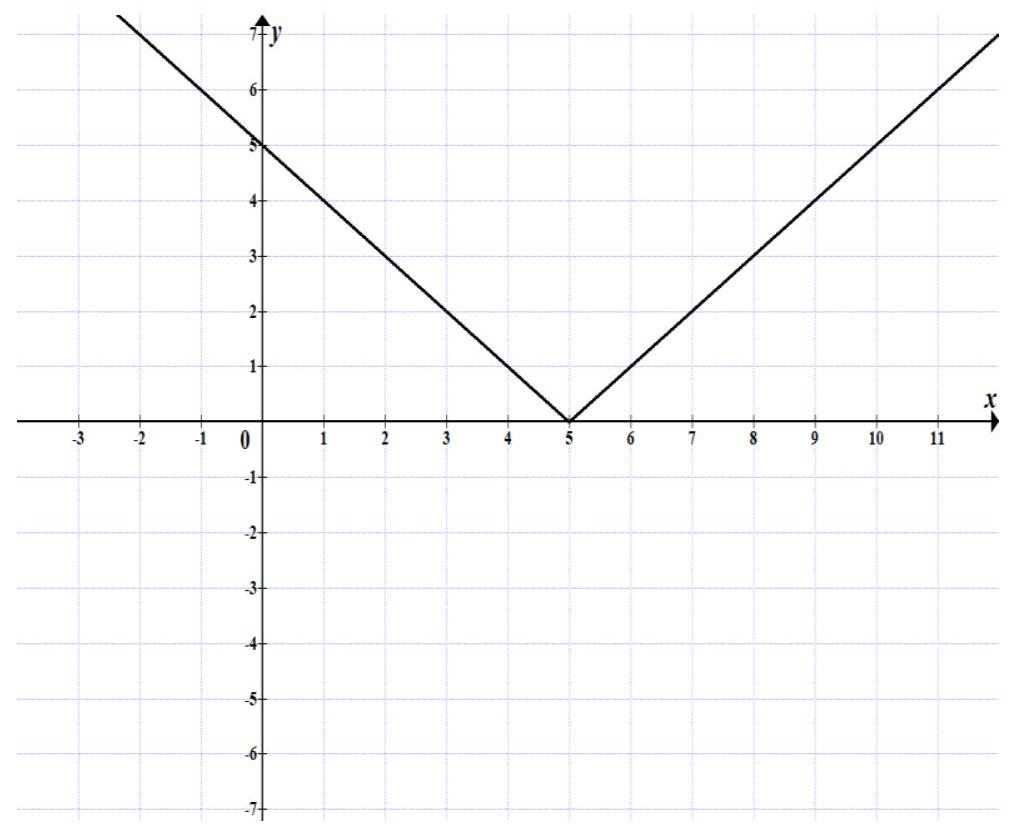
\includegraphics[max width=\textwidth, center]{2025_02_07_176452ab2cb6278af830g-07}

Wnioskujemy stąd, że podane równanie ma dwa pierwiastki dodatnie, jeśli spełniona jest nierówność

$$
0<(a-1)^{2}-4<5 \text {, czyli nierówność } 4<(a-1)^{2}<9 \text {. }
$$

Stąd otrzymujemy, że $2<|a-1|<3$, zatem

$$
(a-1) \in(-3,-2) \cup(2,3) .
$$

Ostatecznie $a \in(-2,-1) \cup(3,4)$.

\section*{II sposób („podstawianie")}
Równanie $|x-5|=(a-1)^{2}-4$ ma dwa dodatnie rozwiązania rzeczywiste, gdy prawdziwa jest nierówność

$$
0<|x-5|<5 .
$$

Ponieważ $|x-5|=(a-1)^{2}-4$, więc prawdziwa jest nierówność

$$
0<(a-1)^{2}-4<5
$$

Nierówność ta jest równoważna koniunkcji nierówności

$$
(a-3)(a+1)>0 \quad \text { i } \quad(a+2)(a-4)<0
$$

skąd otrzymujemy

$$
a \in(-\infty,-1) \cup(3,+\infty) \quad \text { i } \quad a \in(-2,4) .
$$

Zatem dla $a \in(-2,-1) \cup(3,4)$ równanie $|x-5|=(a-1)^{2}-4$ ma dwa rozwiązania dodatnie.

\section*{III sposób}
Równanie $|x-5|=(a-1)^{2}-4$ ma dwa rozwiązania, gdy spełniona jest nierówność

$$
(a-1)^{2}-4>0
$$

Nierówność ta jest równoważna nierówności $(a-3)(a+1)>0$, skąd otrzymujemy


\begin{equation*}
a<-1 \text { lub } a>3 \tag{1}
\end{equation*}


Równanie $|x-5|=(a-1)^{2}-4$ jest równoważne alternatywie równań:

$$
\begin{array}{lll}
x-5=(a-1)^{2}-4 & \text { lub } & x-5=-(a-1)^{2}+4 \\
x=(a-1)^{2}+1 & \text { lub } & x=-(a-1)^{2}+9
\end{array}
$$

Rozwiązanie pierwszego z równań jest liczbą dodatnią, dla każdej liczby rzeczywistej $a$. Zatem, aby równanie miało dwa dodatnie rozwiązania musi być spełniony warunek:

$$
-(a-1)^{2}+9>0
$$

Stąd otrzymujemy $(3+a-1)(3-a+1)>0$, czyli $(a+2)(4-a)>0$, a zatem


\begin{equation*}
-2<a<4 . \tag{2}
\end{equation*}


Uwzględniając (1) i (2) otrzymujemy $a \in(-2,-1) \cup(3,4)$.

\section*{IV sposób}
Ponieważ lewa strona równania $|x-5|=(a-1)^{2}-4$ jest nieujemna, więc równanie ma co najmniej jedno rozwiązanie rzeczywiste wtedy i tylko wtedy, gdy

$$
\begin{gathered}
(a-1)^{2}-4 \geq 0, \\
(a-1-2)(a-1+2) \geq 0, \\
(a-3)(a+1) \geq 0, \\
a \leq-1 \quad \text { lub } \quad a \geq 3 .
\end{gathered}
$$

Podnosząc obie strony równania $|x-5|=(a-1)^{2}-4$ do kwadratu, otrzymujemy równanie równoważne

$$
\begin{gathered}
|x-5|^{2}=\left((a-1)^{2}-4\right)^{2} \\
(x-5)^{2}=\left((a-1)^{2}-4\right)^{2} \\
x^{2}-10 x+25-\left((a-1)^{2}-4\right)^{2}=0
\end{gathered}
$$

Równanie to ma dwa dodatnie rozwiązania rzeczywiste $x_{1}, x_{2}$, gdy spełnione są jednocześnie trzy warunki

$$
\Delta>0 \quad \text { i } \quad x_{1}+x_{2}>0 \quad \text { i } \quad x_{1} x_{2}>0 .
$$

Ze wzorów Viète'a otrzymujemy

$$
(-10)^{2}-4\left(25-\left((a-1)^{2}-4\right)^{2}\right)>0 \quad \text { i } \quad \frac{-(-10)}{1}>0 \quad \text { i } \quad 25-\left((a-1)^{2}-4\right)^{2}>0
$$

Druga z tych nierówności jest prawdziwa dla każdej wartości rzeczywistej a.

Rozwiązujemy pierwszą z tych nierówności

$$
\begin{gathered}
100-4\left(25-\left((a-1)^{2}-4\right)^{2}\right)>0 \\
25-\left(25-\left((a-1)^{2}-4\right)^{2}\right)>0, \\
\left((a-1)^{2}-4\right)^{2}>0 \\
(a-1)^{2}-4 \neq 0 \\
(a-1-2)(a-1+2) \neq 0 \\
(a-3)(a+1) \neq 0 \\
a \neq 3 \quad \text { i } a \neq-1
\end{gathered}
$$

Rozwiązujemy trzecią z nierówności

$$
\begin{gathered}
25-\left((a-1)^{2}-4\right)^{2}>0, \\
\left(5-\left((a-1)^{2}-4\right)\right)\left(5+\left((a-1)^{2}-4\right)\right)>0, \\
\left(9-(a-1)^{2}\right)\left((a-1)^{2}+1\right)>0,
\end{gathered}
$$

Ponieważ $(a-1)^{2}+1>0$ dla każdej wartości $a$, więc

$$
\begin{gathered}
9-(a-1)^{2}>0 \\
(3-(a-1))(3+(a-1))>0, \\
(4-a)(2+a)>0, \\
-2<a<4 .
\end{gathered}
$$

W rezultacie otrzymujemy

$$
(a \leq-1 \text { lub } a \geq 3) \text { i } a \neq 3 \text { i } a \neq-1 \text { i }-2<a<4 .
$$

Stąd $a \in(-2,-1) \cup(3,4)$.

\section*{V sposób}
Rozważmy dwa przypadki.

\begin{enumerate}
  \item Gdy $x-5 \geq 0$, czyli $x \geq 5$, to wtedy $|x-5|=x-5$, a równanie ma postać $x-5=(a-1)^{2}-4$. Stąd $x=(a-1)^{2}+1$. Rozwiązanie to jest dodatnie dla każdej wartości rzeczywistej a. Ponieważ $x \geq 5$, więc $(a-1)^{2}+1 \geq 5$, czyli $(a-1)^{2} \geq 4$, skąd $|a-1| \geq 2$, a więc $a \leq-1$ lub $a \geq 3$. W tym przypadku otrzymujemy
\end{enumerate}

$$
a \in(-\infty,-1\rangle \cup\langle 3,+\infty)
$$

\begin{enumerate}
  \setcounter{enumi}{1}
  \item Gdy $x-5<0$, czyli $x<5$, to wtedy $|x-5|=5-x$, a równanie ma postać $5-x=(a-1)^{2}-4$. Stąd $x=9-(a-1)^{2}$. Rozwiązanie to jest dodatnie, gdy $9-(a-1)^{2}>0$, czyli $(a-1)^{2}<9$, skąd $|a-1|<3$, a więc $-2<a<4$. Rozwiązanie to jest\\
mniejsze od 5 , gdy $9-(a-1)^{2}<5$, czyli $(a-1)^{2}>4$, skąd $|a-1|>2$, a więc $a<-1$ lub $a>3$. Zatem w tym przypadku otrzymujemy $a \in(-2,-1) \cup(3,4)$.
\end{enumerate}

W rezultacie rozpatrzonych przypadków otrzymujemy

$$
a \in(-\infty,-1\rangle \cup\langle 3,+\infty) \text { i } a \in(-2,-1) \cup(3,4)
$$

a więc $a \in(-2,-1) \cup(3,4)$.

\section*{Zadanie 7. (0-3)}
\begin{center}
\begin{tabular}{|c|l|}
\hline
Wymagania ogólne & \multicolumn{1}{c|}{Wymagania szczegółowe} \\
\hline
V. Rozumowanie i argumentacja. & \begin{tabular}{l}
7. Planimetria. Zdający rozpoznaje trójkąty podobne \\
i wykorzystuje (także w kontekstach praktycznych) \\
cechy podobieństwa trójkątów (7.3). \\
\end{tabular} \\
\hline
\end{tabular}
\end{center}

\section*{Zasady oceniania I i ll sposobu}
Rozwiązanie, w którym postęp jest wprawdzie niewielki, ale konieczny na drodze do pełnego rozwiązania zadania 1p. Zdający:

\begin{itemize}
  \item skorzysta z podobieństwa trójkątów i zapisze, np.: $|A D|=3|K P|$ lub
\end{itemize}

$$
|C P|=x \text { i }|D P|=2 x
$$

albo

\begin{itemize}
  \item skorzysta z twierdzenia o odcinkach stycznych i zapisze, np.: $|K M|=|K P|$ i na tym zakończy lub dalej popełni błędy.
\end{itemize}

Pokonanie zasadniczych trudności zadania 2p.\\
Zdający:

\begin{itemize}
  \item skorzysta z podobieństwa trójkątów CPK i CMD i zapisze poprawne równanie pozwalające obliczyć długość odcinka $P K: \frac{|P K|}{2}=\frac{2 x}{3 x}$\\
albo
  \item skorzysta z podobieństwa trójkątów $A D M$ i $A C D$ i zapisze poprawne równanie z jedną niewiadomą, np. $\frac{4-t}{3 t}=\frac{3 t}{6}$, gdzie $t=|K M|=|K P|$\\
i na tym zakończy lub dalej popełni błędy.\\
Rozwiązanie pełne 3p.\\
Zdający rozwiąże powyższe równanie i uzasadni, że $|A M|:|M C|=4: 5$.
\end{itemize}

\section*{Przykładowe rozwiązanie}
\section*{I sposób}
Najpierw uzupełnimy rysunek.\\
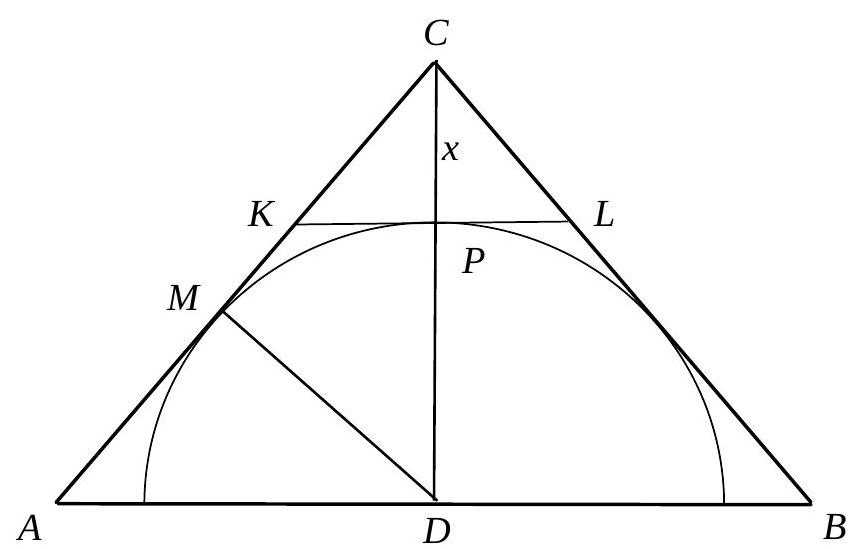
\includegraphics[max width=\textwidth, center]{2025_02_07_176452ab2cb6278af830g-11(1)}

Z twierdzenia odwrotnego do twierdzenia Talesa wnosimy, że odcinek KL jest równoległy do odcinka $A B$.\\
Oznaczmy środek odcinka $K L$ przez $P$ i niech $|C P|=x$.\\
Trójkąty CKP i CAD są podobne (cecha $K K K$ ) w skali 1:3. Wtedy $|P D|=2 x$ i $|M D|=2 x$.\\
Trójkąty CPK i CMD są podobne (cecha $K K K$ ). Stąd $\frac{|P K|}{|C K|}=\frac{|M D|}{|C D|}$, czyli $\frac{|P K|}{2}=\frac{2 x}{3 x}$.\\
Stąd $|P K|=\frac{4}{3}$, więc $|A M|=\frac{8}{3}$ oraz $|M C|=6-\frac{8}{3}=\frac{10}{3}$.\\
Zatem $\frac{|A M|}{|M C|}=\frac{\frac{8}{3}}{\frac{10}{3}}=\frac{4}{5}$.\\
To kończy dowód.

\section*{Il sposób}
Najpierw uzupełnimy rysunek.\\
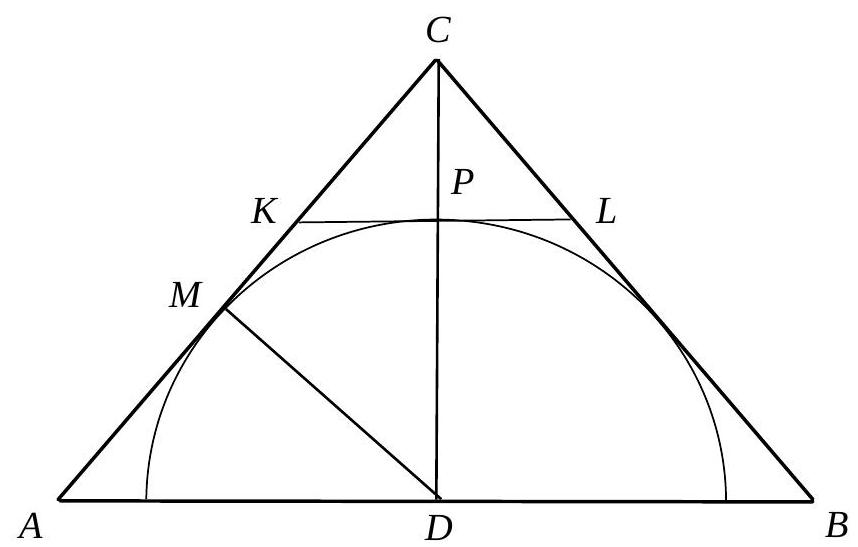
\includegraphics[max width=\textwidth, center]{2025_02_07_176452ab2cb6278af830g-11}

Z twierdzenia odwrotnego do twierdzenia Talesa wnosimy, że odcinek KL jest równoległy do odcinka $A B$.\\
Niech punkt $P$ będzie środkiem odcinka $K L$.\\
Zauważamy, że $|K M|=|K P|$, z twierdzenia o równości odcinków stycznych, łączących punkt leżący poza okręgiem z punktami styczności.

Niech $|K M|=|K P|=t$. Wtedy $|A D|=3 t \mathrm{i}|A M|=4-t$. Trójkąt $A D M$ jest podobny do trójkąta $A C D$, na mocy cechy (kąt, kąt, kąt); są to trójkąty prostokątne, a kąt $M A D$ jest wspólny dla obu trójkątów.

Możemy zatem zapisać równość: $\frac{|A M|}{|A D|}=\frac{|A D|}{|A C|}$, czyli $\frac{4-t}{3 t}=\frac{3 t}{6}$, skąd otrzymujemy równanie $9 t^{2}+6 t-24=0$.\\
Równanie to ma dwa rozwiązania: $t=-2, t=\frac{4}{3}$. Odrzucamy ujemne rozwiązanie tego równania.\\
Zatem $t=\frac{4}{3}$. Ostatecznie $\frac{|A M|}{|M C|}=\frac{4-\frac{4}{3}}{2+\frac{4}{3}}=\frac{\frac{8}{3}}{\frac{10}{3}}=\frac{4}{5}$.\\
To kończy dowód.

\section*{Zadanie 8. (0-3)}
\begin{center}
\begin{tabular}{|c|c|}
\hline
Wymagania ogólne & \multicolumn{1}{c|}{Wymagania szczegółowe} \\
\hline
V. Rozumowanie i argumentacja. & \begin{tabular}{l}
2. Wyrażenia algebraiczne. Zdający używa wzorów \\
skróconego mnożenia $(a \pm b)^{2}$ oraz $a^{2}-b^{2}(2.1)$. \\
\end{tabular} \\
\hline
\end{tabular}
\end{center}

\section*{Zasady oceniania I sposobu rozwiązania}
\begin{verbatim}
Rozwiązanie, w którym postęp jest wprawdzie niewielki, ale konieczny na drodze do pełnego rozwiązania zadania
Zdający zapisze równanie $(a+1)^{2}=(2 b+1)^{2}$
i na tym zakończy lub dalej popełni błędy.
\end{verbatim}

Pokonanie zasadniczych trudności zadania ..... 2p.\\
Zdający zapisze wniosek $a=2 b$ (bez uzasadnienia lub z niepełnym uzasadnieniem) i na tym zakończy lub dalej popełni błędy.\\
Rozwiązanie pełne ..... 3p.

Zdający zapisze pełne uzasadnienie.

\section*{Zasady oceniania II sposobu rozwiązania}
Rozwiązanie, w którym postęp jest wprawdzie niewielki, ale konieczny na drodze do pełnego rozwiązania zadania ..... 1p.

Zdający zapisze równanie $(a-2 b)(a+2 b)=-2(a-2 b)$\\
i na tym zakończy lub dalej popełni błędy.\\
Pokonanie zasadniczych trudności zadania ..... 2p.\\
Zdający zapisze wniosek $a=2 b$ (bez uzasadnienia lub z niepełnym uzasadnieniem) i na tym zakończy lub dalej popełni błędy.\\
Rozwiązanie pełne ..... 3p.\\
Zdający zapisze pełne uzasadnienie.\\
Zasady oceniania III sposobu rozwiązania\\
Rozwiązanie, w którym postęp jest wprawdzie niewielki, ale konieczny na drodze do pełnego rozwiązania zadania ..... 1p.\\
Zdający obliczy wyróżnik trójmianu kwadratowego $a^{2}+2 a-4 b^{2}-4 b$ np. zmiennej $a$,$\Delta=(4 b+2)^{2}$ i zapisze, że jest on nieujemny dla każdej wartości $b$ albo, że jest on dodatnidla każdej wartości $b>0$i na tym zakończy lub dalej popełni błędy.\\
Pokonanie zasadniczych trudności zadania ..... 2p.\\
Zdający obliczy pierwiastki trójmianu $a^{2}+2 a-4 b^{2}-4 b: a=-2-2 b$ lub $a=2 b$i na tym zakończy lub dalej popełni błędy.\\
Rozwiązanie pełne ..... $3 p$.\\
Zdający zapisze pełne uzasadnienie.

\section*{Uwaga}
Jeżeli zdający sprawdza prawdziwość równania jedynie dla wybranych wartości a i $b$, to otrzymuje 0 punktów.

\section*{Przykładowe rozwiązania}
\section*{I sposób}
Zapisujemy równanie równoważne równaniu z założenia: $a^{2}+2 a+1=4 b^{2}+4 b+1$.\\
Korzystamy ze wzoru skróconego mnożenia i zapisujemy to równanie w postaci $(a+1)^{2}=(2 b+1)^{2}$. Oba wyrażenia w nawiasach są dodatnie, zatem równość kwadratów jest równoważna równości tych wyrażeń, stąd $a+1=2 b+1$ i dalej, $a=2 b$.

\section*{To kończy dowód.}
\section*{Il sposób}
Przekształcamy założenie równoważnie:

$$
\begin{gathered}
a^{2}-4 b^{2}=4 b-2 a . \\
(a-2 b)(a+2 b)=-2(a-2 b) \\
(a-2 b)(a+2 b+2)=0 .
\end{gathered}
$$

Liczby $a$ i $b$ są dodatnie, zatem $a+2 b+2 \neq 0$. Stąd $a-2 b=0$, czyli $a=2 b$.

\section*{To kończy dowód.}
\section*{III sposób}
Wyrażenie $a^{2}+2 a-4 b^{2}-4 b$ traktujemy jako trójmian kwadratowy jednej zmiennej np. a.\\
Wyróżnik trójmianu kwadratowego $a^{2}+2 a-4 b^{2}-4 b$ jest równy: $\Delta=(4 b+2)^{2}$.\\
Ten wyróżnik jest nieujemny dla każdej rzeczywistej wartości $b$.\\
Obliczamy pierwiastki tego trójmianu

$$
a=-2-2 b \text { lub } a=2 b .
$$

Ponieważ $b>0$, więc liczba $-2-2 b<0$, co jest sprzeczne z założeniem, że $a>0$.\\
Zatem $a=2 b$.

\section*{To kończy dowód.}
\section*{Zadanie 9. (0-4)}
\begin{center}
\begin{tabular}{|c|l|}
\hline
\multicolumn{1}{|c|}{Wymagania ogólne} & \multicolumn{1}{c|}{Wymagania szczegółowe} \\
\hline
IV. Użycie i tworzenie strategii. & \begin{tabular}{l}
6. Trygonometria. Zdający rozwiązuje równania \\
i nierówności trygonometryczne (R6.6). \\
\end{tabular} \\
\hline
\end{tabular}
\end{center}

\section*{Zasady oceniania \\
 Rozwiązanie, w którym postęp jest niewielki, ale konieczny na drodze do pełnego rozwiązania \\
 1p.}
Zdający doprowadzi równanie do postaci równoważnej, w której występuje tylko jedna funkcja trygonometryczna tego samego kąta, np.: $3-6 \sin ^{2} x+10-10 \sin ^{2} x=24 \sin x-3$

\section*{i na tym zakończy lub dalej popełni błędy}
Rozwiązanie, w którym jest istotny postęp 2p.\\
Zdający rozwiąże równanie kwadratowe $2 t^{2}+3 t-2=0: t=-2$ oraz $t=\frac{1}{2}$\\
i na tym zakończy lub dalej popełni błędy.\\
Pokonanie zasadniczych trudności zadania 3 p.

\section*{Zdający}
\begin{itemize}
  \item zapisze, że równanie $\sin x=-2$ nie ma rozwiązań i poda co najmniej jedną serię rozwiązań równania $\sin x=\frac{1}{2} \mathrm{w}$ zbiorze liczb rzeczywistych:
\end{itemize}

$$
x=\frac{\pi}{6}+2 k \pi \quad \text { lub } \quad x=\frac{5 \pi}{6}+2 k \pi \text {, gdzie } k \text { jest liczbą całkowitą }
$$

albo

\begin{itemize}
  \item zapisze, że równanie $\sin x=-2$ nie ma rozwiązań i poda jedno rozwiązanie równania $\sin x=\frac{1}{2} w$ przedziale $\langle 0,2 \pi\rangle$\\
i na tym zakończy lub dalej popełni błędy\\
Rozwiązanie pełne. 4 p.
\end{itemize}

Zdający wyznaczy oba rozwiązania równania: $x_{1}=\frac{\pi}{6}$ oraz $x_{2}=\frac{5 \pi}{6}$.

\section*{Uwagi}
\begin{enumerate}
  \item Akceptujemy przybliżone rozwiązania elementarnych równań trygonometrycznych.
  \item Jeżeli zdający wyznaczy poprawnie obydwa rozwiązania równania $\sin x=\frac{1}{2}$ należące do przedziału $(0,2 \pi)$ i nie zapisze komentarza dotyczącego równania $\sin x=-2$, to otrzymuje 4 punkty.
  \item Jeżeli zdający przed uzyskaniem trygonometrycznych równań elementarnych popełni błędy rachunkowe i otrzyma równania elementarne, z których co najmniej jedno ma dwie serie rozwiązań w zbiorze liczb rzeczywistych, to otrzymuje co najwyżej 3 punkty za całe rozwiązanie.
  \item Jeżeli zdający przed uzyskaniem elementarnych równań trygonometrycznych popełni błąd polegający na niepoprawnym zastosowaniu wzoru na cosinus kąta podwojonego lub błąd polegający na podstawieniu $w$ miejsce $\sin x$ wyrażenia $\sqrt{1-\cos ^{2} x}$, ale otrzyma co najmniej jedno równanie typu $\sin x=a$, gdzie $a \in(-1,0) \cup(0,1)$, i konsekwentnie to równanie rozwiąże, to za całe rozwiązanie może otrzymać co najwyżej 2 punkty. Jeżeli jednak zdający otrzyma co najmniej jedno równanie typu $\sin x=a$, gdzie $a \in\{-1,0,1\}$, i to równanie konsekwentnie rozwiąże, to za całe rozwiązanie może otrzymać co najwyżej 1 punkt.
  \item Jeżeli zdający zapisze równanie $\sin x=\frac{2}{3} \cos ^{2} x$, równoważne równaniu $3 \cos 2 x+10 \cos ^{2} x=24 \sin x-3$, a następnie rozwiąże równanie $\frac{4}{9} \cos ^{4} x+\cos ^{2} x-1=0$, otrzymując 4 rozwiązania tego równania należące do przedziału $\langle 0,2 \pi\rangle: x=\frac{\pi}{6}$, $x=\frac{5}{6} \pi, x=\frac{7}{6} \pi, x=\frac{11}{6} \pi$ i nie odrzuci „obcych" rozwiązań: $x=\frac{7}{6} \pi, x=\frac{11}{6} \pi$, to za całe rozwiązanie może otrzymać co najwyżej 2 punkty.
\end{enumerate}

\section*{Przykładowe rozwiązanie}
Przekształcamy dane równanie w sposób równoważny:

$$
\begin{gathered}
3 \cos 2 x+10 \cos ^{2} x=24 \sin x-3, \\
3\left(1-2 \sin ^{2} x\right)+10\left(1-\sin ^{2} x\right)=24 \sin x-3, \\
3-6 \sin ^{2} x+10-10 \sin ^{2} x=24 \sin x-3, \\
16-16 \sin ^{2} x=24 \sin x, \\
16 \sin ^{2} x+24 \sin x-16=0 \\
2 \sin ^{2} x+3 \sin x-2=0
\end{gathered}
$$

Niech $t=\sin x$. Rozwiązujemy równanie kwadratowe:

$$
\begin{gathered}
2 t^{2}+3 t-2=0, \\
\Delta=3^{2}+4 \cdot 2 \cdot 2=9+16=25, \\
\sqrt{\Delta}=5,
\end{gathered}
$$

$$
\begin{gathered}
t_{1}=\frac{-3-5}{4}=\frac{-8}{4}=-2, \\
t_{2}=\frac{-3+5}{4}=\frac{2}{4}=\frac{1}{2} .
\end{gathered}
$$

Równanie $\sin x=-2$ jest sprzeczne, a równanie $\sin x=\frac{1}{2}$ ma w przedziale $\langle 0,2 \pi\rangle$ dwa rozwiązania: $x_{1}=\frac{\pi}{6}$ oraz $x_{2}=\frac{5 \pi}{6}$.

\section*{Zadanie 10. (0-5)}
\begin{center}
\begin{tabular}{|c|l|}
\hline
\multicolumn{1}{|c|}{Wymagania ogólne} & \multicolumn{1}{c|}{Wymagania szczegółowe} \\
\hline
V. Rozumowanie i argumentacja. & \begin{tabular}{l}
5. Ciągi. Zdający stosuje wzór na $n$-ty wyraz i na \\
sumę $n$-początkowych wyrazów ciągu \\
aryytetycznego (5.3). Zdaący stosuje wzór na $n$-ty \\
wyraz i na sumę $n$-początkowych wyrazów ciągu \\
geometrycznego (5.4). \\
\end{tabular} \\
\hline
\end{tabular}
\end{center}

\section*{Zasady oceniania I, II i III sposobu rozwiązania \\
 Rozwiązanie, w którym postęp jest wprawdzie niewielki, ale konieczny na drodze do pełnego rozwiązania zadania \\
 1p.}
Zdający

\begin{itemize}
  \item wykorzysta wzór na n-ty wyraz ciągu geometrycznego lub własność ciągu geometrycznego i zapisze np.:
\end{itemize}

$$
a_{2}=a_{1} q \text { i } a_{3}=a_{1} q^{2}
$$

lub

$$
a_{1}+a_{1} q+a_{1} q^{2}=\frac{21}{4}
$$

lub

$$
a_{2}^{2}=a_{1} \cdot a_{3}
$$

albo

\begin{itemize}
  \item wykorzysta wzór na $n$-ty wyraz ciągu arytmetycznego lub własność ciągu arytmetycznego i zapisze np.:
  \item $\left(a_{2}=a_{3}+r\right.$ i $\left.a_{1}=a_{3}+3 r\right)$ lub $\left(b_{2}=a_{3}+r\right.$ i $\left.b_{4}=a_{3}+3 r\right)$ lub $\left(b_{2}=b_{1}+r\right.$ i $\left.b_{4}=b_{1}+3 r\right)$\\
lub
  \item $a_{1}-a_{2}=2\left(a_{2}-a_{3}\right)$ lub $b_{4}-b_{2}=2\left(b_{2}-b_{1}\right)$\\
lub
\end{itemize}

$$
\text { - } \quad b_{3}=\frac{b_{4}+b_{2}}{2} \quad \text { i } b_{2}=\frac{b_{1}+b_{3}}{2}
$$

i na tym zakończy lub dalej popełni błędy.\\
Rozwiązanie, w którym jest istotny postęp\\
Zdający

\begin{itemize}
  \item zapisze układ równań, z którego można otrzymać równanie z jedną niewiadomą, np.:
\end{itemize}

$$
\text { - } \quad a_{1}+a_{1} q+a_{1} q^{2}=\frac{21}{4} \text { i } a_{1}=a_{1} q^{2}+3\left(a_{1} q-a_{1} q^{2}\right)
$$

lub

$$
a_{1}+a_{1} q+a_{1} q^{2}=\frac{21}{4} \text { i } a_{1} q=\frac{\frac{a_{1}+a_{1} q}{2}+a_{1} q^{2}}{2}
$$

albo

\begin{itemize}
  \item zapisze równanie pozwalające wyznaczyć związek między $a_{3} \mathrm{i} r$, np.:
\end{itemize}

$$
\left(a_{3}+r\right)^{2}=\left(a_{3}+3 r\right) \cdot a_{3}
$$

i na tym zakończy lub dalej popełni błędy.

\section*{Pokonanie zasadniczych trudności zadania}
\section*{Zdający}
\begin{itemize}
  \item zapisze równanie $z$ jedną niewiadomą, np.: $2 q^{2}-3 q+1=0$\\
albo
  \item zapisze $r=a_{3}$\\
i na tym zakończy lub dalej popełni błędy.
\end{itemize}

\section*{Rozwiązanie prawie pełne 4p.}
\section*{Zdający}
\begin{itemize}
  \item rozwiąże równanie $z$ jedną niewiadomą, np. $2 q^{2}-3 q+1=0: q=1$ lub $q=\frac{1}{2}$\\
albo
  \item obliczy trzeci wyraz ciągu geometrycznego $\left(a_{n}\right): a_{3}=\frac{3}{4}$\\
i na tym zakończy lub dalej popełni błędy.\\
Rozwiązanie pełne\\
5 p.\\
Zdający obliczy pierwszy wyraz ciągu geometrycznego $a_{1}=3$.
\end{itemize}

\section*{Uwagi}
\begin{enumerate}
  \item Jeżeli zdający rozwiąże równanie $z$ jedną niewiadomą, np. $2 q^{2}-3 q+1=0: q=1$ lub $q=\frac{1}{2}$ oraz obliczy dwie wartości $a_{1}: a_{1}=3, a_{1}=\frac{7}{4}$ i nie odrzuci $a_{1}=\frac{7}{4}$, to otrzymuje 4 punkty.
  \item Jeśli zdający stosuje poprawną strategię rozwiązania zadania, a jedynymi błędami w rozwiązaniu są błędy rachunkowe, to otrzymuje maksymalnie 4 punkty.
  \item Jeśli zdający błędnie stosuje wzór na $n$-ty wyraz ciągu geometrycznego (np. zapisuje $a_{3}=a_{1} q^{3}$ ) lub ciągu arytmetycznego i korzysta $z$ tego w rozwiązaniu, to za całe rozwiązanie może otrzymać co najwyżej 3 punkty.
  \item Jeśli zdający odgadnie iloraz ciągu geometrycznego, a następnie obliczy na tej podstawie pierwszy wyraz tego ciągu, to otrzymuje 1 punkt za całe rozwiązanie.
  \item Jeśli zdający zamienia (myli) własności ciągu geometrycznego $z$ własnościami ciągu arytmetycznego, to za całe rozwiązanie otrzymuje 0 punktów.
  \item Jeśli zdający zapisuje tylko odpowiedź $a_{1}=3$, to otrzymuje $\mathbf{0}$ punktów.
  \item Akceptujemy sytuacje, w których zdający dzieli obie strony zbudowanych przez siebie równań przez $a_{1}$ albo przez $r$, albo też przez $q-1$ bez zapisania jakiegokolwiek komentarza.
\end{enumerate}

\section*{Przykładowe rozwiązania}
\section*{I sposób}
Sumując wyrazy ciągu geometrycznego otrzymujemy równość


\begin{equation*}
a_{1}+a_{1} q+a_{1} q^{2}=\frac{21}{4} . \tag{1}
\end{equation*}


Niech $\left(b_{n}\right)$ będzie rosnącym ciągiem arytmetycznym.\\
Zatem $b_{1}=a_{1} q^{2}, b_{2}=a_{1} q, b_{4}=a_{1}$, więc różnica tego ciągu $r=a_{1} q-a_{1} q^{2}$ oraz $b_{4}=b_{1}+3 r$, czyli $a_{1}=a_{1} q^{2}+3\left(a_{1} q-a_{1} q^{2}\right)$.\\
Stąd wynika, że $a_{1}=3 a_{1} q-2 a_{1} q^{2}$ i $a_{1}\left(2 q^{2}-3 q+1\right)=0$.\\
Ponieważ z równości (1) wynika, że $a_{1} \neq 0$, więc $2 q^{2}-3 q+1=0$. Zatem $q=1$ lub $q=\frac{1}{2}$.\\
Dla $q=1$ ciąg $\left(a_{n}\right)$ jest stały. Stąd ciąg $\left(b_{n}\right)$ też jest stały. Zatem tylko dla $q=\frac{1}{2}$ ciąg $\left(b_{n}\right)$ może być ciągiem rosnącym. Otrzymujemy wtedy $r=\frac{1}{4} a_{1}$. Z równości (1) otrzymujemy $a_{1}+\frac{1}{2} a_{1}+\frac{1}{4} a_{1}=\frac{21}{4}$, a stąd wynika, że $a_{1}=3$.

\section*{Il sposób}
W ciągu arytmetycznym $b_{1}=a_{3}, b_{2}=a_{3}+r, b_{4}=a_{3}+3 r$, gdzie $r>0$.\\
Ponieważ ciąg $\left(a_{3}+3 r, a_{3}+r, a_{3}\right)$ jest ciągiem geometrycznym, więc zachodzi równość

$$
\left(a_{3}+r\right)^{2}=\left(a_{3}+3 r\right) \cdot a_{3},
$$

skąd wynika, że $a_{3}^{2}+2 a_{3} r+r^{2}=a_{3}^{2}+3 a_{3} r$,\\
a zatem $r^{2}=a_{3} r$.\\
Ponieważ z założenia $r>0$, więc $r=a_{3}$. Podana suma trzech wyrazów jest zatem równa

$$
4 a_{3}+2 a_{3}+a_{3}=\frac{21}{4} .
$$

Otrzymujemy zatem $a_{3}=\frac{3}{4}$. Wtedy $a_{1}=b_{4}=4 a_{3}=3$.

\section*{Ill sposób}
$Z$ danych w treści zadania wynikają równości:

$$
b_{1}=a_{1} q^{2}, b_{2}=a_{1} q, b_{4}=a_{1} .
$$

Ponieważ $\left(b_{n}\right)$ jest ciągiem arytmetycznym, więc możemy zapisać równości

$$
b_{3}=\frac{b_{4}+b_{2}}{2}=\frac{a_{1}+a_{1} q}{2}
$$

oraz

$$
b_{2}=\frac{b_{3}+b_{1}}{2}=\frac{\frac{a_{1}+a_{1} q}{2}+a_{1} q^{2}}{2}=a_{1} q
$$

Rozwiążemy równanie

$$
\frac{\frac{a_{1}+a_{1} q}{2}+a_{1} q^{2}}{2}=a_{1} q
$$

Ponieważ $a_{1}+a_{1} q+a_{1} q^{2}=\frac{21}{4}$, więc możemy założyć, że $a_{1} \neq 0$. Powyższe równanie jest zatem równoważne równaniu

$$
\frac{\frac{1+q}{2}+q^{2}}{2}=q \text {, czyli równaniu } 1+q+2 q^{2}=4 q \text {. }
$$

Równanie kwadratowe $2 q^{2}-3 q+1=0$ ma dwa rozwiązania: $q=1$ oraz $q=\frac{1}{2}$.\\
Jeśli $q=1$, to obydwa ciągi są ciągami stałymi. Zatem tylko dla $q=\frac{1}{2}$ ciąg $\left(b_{n}\right)$ może być ciągiem rosnącym.\\
Z równości $a_{1}+a_{1} q+a_{1} q^{2}=\frac{21}{4}$ otrzymujemy równanie $\frac{7}{4} a_{1}=\frac{21}{4}$, czyli $a_{1}=3$.

\section*{Zadanie 11. (0-4)}
\begin{center}
\begin{tabular}{|c|l|}
\hline
Wymagania ogólne & \multicolumn{1}{c|}{Wymagania szczegółowe} \\
\hline
III. Modelowanie matematyczne. & \begin{tabular}{l}
3. Równania i nierówności. Zdający stosuje wzory \\
Viète'a (R3.1). \\
\end{tabular} \\
\hline
\end{tabular}
\end{center}

\section*{Zasady oceniania I i II sposobu}
Rozwiązanie zadania składa się z dwóch części.\\
Pierwsza z nich polega na:

\begin{itemize}
  \item rozwiązaniu nierówności $\Delta>0: m \in R \backslash\{8\}$\\
albo
  \item sprawdzeniu, że dla każdej obliczonej wartości parametru $m$ równanie $x^{2}-(3 m+2) x+2 m^{2}+7 m-15=0$ ma dwa rozwiązania rzeczywiste.\\
Za poprawne rozwiązanie tej części zdający otrzymuje 1 punkt.\\
Druga część polega na wyznaczeniu tych wartości parametru $m$, dla których jest spełniony warunek $2 x_{1}^{2}+5 x_{1} x_{2}+2 x_{2}^{2}=2$. Za tę część rozwiązania zdający otrzymuje 3 punkty.\\
Podział punktów za drugą część rozwiązania:\\
1 punkt zdający otrzymuje za:
  \item obliczenie dwóch pierwiastków trójmianu $x^{2}-(3 m+2) x+2 m^{2}+7 m-15$ :
\end{itemize}

$$
x_{1}=m+5 \text { oraz } x_{2}=2 m-3 .
$$

albo

\begin{itemize}
  \item przekształcenie wyrażenia $2 x_{1}^{2}+5 x_{1} x_{2}+2 x_{2}^{2}$ do postaci: $2\left(x_{1}+x_{2}\right)^{2}+x_{1} x_{2}$\\
lub równoważnej, ale zawierającej jedynie zmienne $x_{1}+x_{2}$ oraz $x_{1} \cdot x_{2}$.\\
2 punkty zdający otrzymuje za:
  \item zapisanie równania $2 x_{1}^{2}+5 x_{1} x_{2}+2 x_{2}^{2}=2$ w postaci równania z jedną niewiadomą $m$, np .:
\end{itemize}

$$
2(m+5)^{2}+5(m+5)(2 m-3)+2(2 m-3)^{2}=2
$$

\section*{albo}
\begin{itemize}
  \item zapisanie równania $2\left(x_{1}+x_{2}\right)^{2}+x_{1} x_{2}=2 \mathrm{w}$ postaci równania z jedną niewiadomą $m$,
\end{itemize}

$$
\mathrm{np} .: 2(3 m+2)^{2}+2 m^{2}+7 m-15=2 \text {. }
$$

3 punkty zdający otrzymuje za rozwiązanie równania $20 m^{2}+31 m-9=0$ :

$$
m_{1}=-\frac{9}{5} \text { oraz } m_{2}=\frac{1}{4} .
$$

\section*{Uwagi}
\begin{enumerate}
  \item Jeżeli zdający zamienia wzory Viète'a przy przekształcaniu lewej strony równania $2 x_{1}^{2}+5 x_{1} x_{2}+2 x_{2}^{2}=2$, to za całe rozwiązanie może otrzymać co najwyżej 2 punkty.
  \item Jeżeli zdający rozpatruje warunek $\Delta \geq 0$ i nie sprawdzi, że dla każdej $z$ otrzymanych wartości parametru $m$ równanie ma dwa rozwiązania rzeczywiste, to może otrzymać co najwyżej 3 punkty za całe rozwiązanie.
  \item Jeżeli zdający przekształci warunek $2 x_{1}^{2}+5 x_{1} x_{2}+2 x_{2}^{2}=2$, otrzyma $2\left(x_{1}+x_{2}\right)^{2}+3 x_{1} x_{2}=2$ i rozwiąże zadanie konsekwentnie do końca, to za drugą część rozwiązania może otrzymać co najwyżej 2 punkty.
  \item Jeżeli zdający wykorzystuje niepoprawny wzór „kwadrat sumy dwóch wyrażeń jest równy sumie kwadratów tych wyrażeń", przekształci warunek $2 x_{1}^{2}+5 x_{1} x_{2}+2 x_{2}^{2}=2$ do postaci $2\left(x_{1}+x_{2}\right)^{2}+5 x_{1} x_{2}=2$, i rozwiąże zadanie konsekwentnie do końca, to za drugą część rozwiązania może otrzymać co najwyżej 1 punkt.
  \item Jeżeli zdający rozpatrując równość $2 x_{1}^{2}+5 x_{1} x_{2}+2 x_{2}^{2}=2$ zmieni liczbę po prawej stronie i zapisze równanie, wynikające ze wzorów Viete'a, w postaci $2(3 m+2)+2 m^{2}+7 m-15=0$, pomijając wykładnik 2 potęgi o podstawie $(3 m+2)$, to za drugą część rozwiązania zadania może otrzymać co najwyżej 1 punkt.
\end{enumerate}

\section*{Przykładowe rozwiązania}
\section*{I sposób}
\begin{enumerate}
  \item Równanie ma dwa różne rozwiązania, gdy wyróżnik trójmianu jest dodatni: $\Delta>0$.
\end{enumerate}

Obliczamy wyróżnik trójmianu:

$$
\begin{aligned}
& \Delta=(-(3 m+2))^{2}-4\left(2 m^{2}+7 m-15\right)=m^{2}-16 m+64=(m-8)^{2} . \\
&(m-8)^{2}>0, \text { gdy } m \neq 8 .
\end{aligned}
$$

Stąd wynika, że trójmian ma następujące pierwiastki: $x_{1}=m+5$ oraz $x_{2}=2 m-3$.\\
Mamy zatem rozwiązać równanie

$$
2(m+5)^{2}+5(m+5)(2 m-3)+2(2 m-3)^{2}=2 .
$$

To równanie doprowadzamy do postaci równoważnej:

$$
20 m^{2}+31 m-9=0 .
$$

Ma ono dwa rozwiązania: $m_{1}=-\frac{9}{5}$ oraz $m_{2}=\frac{1}{4}$\\
Każde z otrzymanych rozwiązań jest różne od 8.\\
Warunki zadania spełniają dwie wartości parametru $m$ : $m_{1}=-\frac{9}{5}$ oraz $m_{2}=\frac{1}{4}$.

\section*{Il sposób}
Przekształcamy równość $2 x_{1}^{2}+5 x_{1} x_{2}+2 x_{2}^{2}=2 \mathrm{w}$ sposób równoważny:

$$
\begin{gathered}
2\left(x_{1}^{2}+x_{2}^{2}\right)+5 x_{1} x_{2}=2, \\
2\left(\left(x_{1}+x_{2}\right)^{2}-2 x_{1} x_{2}\right)+5 x_{1} x_{2}=2, \\
2\left(x_{1}+x_{2}\right)^{2}+x_{1} x_{2}=2 .
\end{gathered}
$$

Ze wzorów Viète'a wynika, że

$$
x_{1}+x_{2}=3 m+2 \text { oraz } x_{1} x_{2}=2 m^{2}+7 m-15,
$$

o ile pierwiastki $x_{1}$ i $x_{2}$ trójmianu istnieja.\\
Mamy zatem rozwiązać równanie

$$
2(3 m+2)^{2}+2 m^{2}+7 m-15=2 .
$$

To równanie doprowadzamy do postaci równoważnej

$$
20 m^{2}+31 m-9=0
$$

Ma ono dwa rozwiązania:

$$
m_{1}=-\frac{9}{5} \text { oraz } m_{2}=\frac{1}{4} .
$$

Pozostaje sprawdzić, czy dla tych wartości $m$ dany trójmian kwadratowy ma dwa różne pierwiastki. Możemy, tak jak w sposobie pierwszym, obliczyć wyróżnik i przekonać się, że jest on nieujemny. Możemy także podstawić znalezione wartości parametru $m$ do danego trójmianu i przekonać się, że otrzymane trójmiany mają dwa różne pierwiastki. Po podstawieniu $m=-\frac{9}{5}$ otrzymamy trójmian:

$$
x^{2}+\frac{17}{5} x-\frac{528}{25}
$$

Po podstawieniu $m=\frac{1}{4}$ otrzymamy trójmian:

$$
x^{2}+\frac{11}{4} x-\frac{105}{8} .
$$

Oba trójmiany mają dwa różne pierwiastki. Można się o tym przekonać, obliczając wyróżniki lub zauważając, że oba trójmiany mają dodatni współczynnik przy $x^{2} i \quad u j e m n y ~ w y r a z ~ w o l n y . ~$

Warunki zadania spełniają dwie wartości parametru $m$ :

$$
m_{1}=-\frac{9}{5} \text { oraz } m_{2}=\frac{1}{4} .
$$

\section*{Zadanie 12. (0-5)}
\begin{center}
\begin{tabular}{|l|l|}
\hline
\multicolumn{1}{|c|}{Wymagania ogólne} & \multicolumn{1}{c|}{Wymagania szczegółowe} \\
\hline
IV. Użycie i tworzenie strategii. & \begin{tabular}{l}
7. Planimetria. Zdający znajduje obrazy niektórych \\
figur geometrycznych w jednokładności (odcinka, \\
trójkąta, czworokąta itp.) (R7.3). \\
 \\
 \\
 \\
 \\
 \\
 \\
 \\
 \\
Z. Geometria na płaszczyźnie kartezjańskiej. \\
$(x-a)^{2}+(y-b)^{2}=r^{2}$ oraz opisuje koła za pomocą \\
nierówności (R8.5). \\
\hline
\end{tabular} \\
\hline
\end{tabular}
\end{center}

\section*{Zasady oceniania I, II, III, IV i V sposobu rozwiązania}
Rozwiązanie składa się z dwóch etapów.\\
Pierwszy etap polega na wyznaczeniu współrzędnych środka danego okręgu. Za poprawne rozwiązanie tego etapu zdający otrzymuje 1 punkt.

Drugi etap polega na wyznaczeniu równania/układu równań prowadzących do wyznaczenia współrzędnych środka jednokładności oraz współrzędnych środka obrazu danego okręgu w tej jednokładności.\\
Za poprawne rozwiązanie tego etapu zdający otrzymuje 4 punkty.

\section*{Podział punktów za pierwszy etap rozwiązania}
Zdający otrzymuje 1 punkt, gdy

\begin{itemize}
  \item zapisze współrzędne środka: $P=(4,3)$\\
lub
  \item zapisze równanie okręgu $x^{2}+y^{2}-8 x-6 y+8=0 \mathrm{w}$ postaci $(x-4)^{2}+(y-3)^{2}=17$.
\end{itemize}

\section*{Podział punktów za drugi etap rozwiązania}
Zdający otrzymuje\\
1 punkt, gdy

\begin{itemize}
  \item obliczy i zapisze współrzędne punktów $K$ i $L: K=(3,7)$ i $L=(8,2)$\\
albo
  \item obliczy odległość punktu $P$ od prostej o równaniu $x+y-10=0: d=|S P|=\frac{3 \sqrt{2}}{2}$\\
albo
  \item zapisze równanie prostej przechodzącej przez punkt $P=(4,3)$ prostopadłej do prostej $x+y-10=0: x-y-1=0$\\
albo
  \item poda tylko promień obrazu okręgu: $R=3 \sqrt{17}$,\\
i na tym zakończy lub dalej popełni błędy.
\end{itemize}

\section*{Zdający otrzymuje}
2 punkty, gdy

\begin{itemize}
  \item zapisze współrzędne środka jednokładności: $S=\left(\frac{11}{2}, \frac{9}{2}\right)$\\
albo
  \item zapisze $P^{\prime}=(x, x-1)$ i zapisze $\left|S P^{\prime}\right|=3 \cdot|S P|=\frac{9 \sqrt{2}}{2}$\\
i na tym zakończy lub dalej popełni błędy.\\
Zdający otrzymuje\\
3 punkty, gdy
  \item zapisze równanie, wynikające z równości $\overrightarrow{S P^{\prime}}=-3 \cdot \overrightarrow{S P}$, prowadzące do wyznaczenia współrzędnych środka $P^{\prime}=(a, b)$ okręgu, będącego obrazem punktu $P=(4,3)$ w jednokładności:
\end{itemize}

$$
\left[a-\frac{11}{2}, b-\frac{9}{2}\right]=-3 \cdot\left[4-\frac{11}{2}, 3-\frac{9}{2}\right]
$$

albo

\begin{itemize}
  \item wykona poprawne podstawienie do odpowiedniego wzoru w zestawie Wybranych wzorów matematycznych i zapisze:
\end{itemize}

$$
a=-3 \cdot 4+(1-(-3)) \cdot \frac{11}{2} \text { oraz } b=-3 \cdot 3+(1-(-3)) \cdot \frac{9}{2}
$$

albo

\begin{itemize}
  \item zapisze równanie, wynikające z równości $\overrightarrow{P P^{\prime}}=-4 \cdot \overrightarrow{S P}$, prowadzące do wyznaczenia współrzędnych środka $P^{\prime}=(a, b)$ okręgu, będącego obrazem punktu $P=(4,3)$ w tej jednokładności:
\end{itemize}

$$
[a-4, b-3]=-4 \cdot\left[4-\frac{11}{2}, 3-\frac{9}{2}\right]
$$

albo

\begin{itemize}
  \item zapisze równanie $\sqrt{(a-4)^{2}+(a-1-3)^{2}}=6 \sqrt{2}$\\
albo
  \item zapisze równanie $\frac{|a+a-1-10|}{\sqrt{2}}=\frac{9 \sqrt{2}}{2}$\\
i na tym zakończy lub dalej popełni błędy.\\
Zdający otrzymuje\\
4 punkty, gdy zapisze równanie szukanego okręgu
\end{itemize}

$$
(x-10)^{2}+(y-9)^{2}=153 .
$$

\section*{Uwagi:}
\begin{enumerate}
  \item Jeśli zdający realizuje poprawną strategię rozwiązania zadania, a jedynymi błędami w rozwiązaniu są błędy rachunkowe, to za takie rozwiązanie otrzymuje co najwyżej 4 punkty.
  \item Jeśli zdający zakłada błędnie, że środkiem jednokładności jest środek danego okręgu, to może otrzymać co najwyżej 1 punkt za drugą część rozwiązania.
  \item Jeśli zdający podczas obliczania wspótrzędnych punktów $K$, $L$ lub $S$ popełnia błąd polegający na zamianie wspótrzędnych i konsekwentnie do tego błędu rozwiąże zadanie do końca, to otrzymuje co najwyżej 4 punkty.
  \item Jeśli zdający stosuje błędne równanie $\overrightarrow{S P}=-3 \cdot \overrightarrow{S P^{\prime}}$ i konsekwentnie do tego błędu rozwiąże zadanie do końca, to otrzymuje co najwyżej 2 punkty za drugą część rozwiązania.
  \item Jeśli zdający zakłada błędnie, że trójkąt $K L P$ jest trójkątem prostokątnym i w rozwiązaniu stosuje tę własnośś, to może otrzymać co najwyżej 2 punkty za drugą część rozwiązania.
  \item Jeżeli zdający narysuje w układzie współrzędnych dany okrąg i daną prostą, a następnie wyznaczy graficznie obraz środka $P^{\prime}$ danego okręgu w jednokładności o środku S i skali $k=-3$ oraz zapisze równanie tego otrzymanego okręgu, to może otrzymać 4 punkty za drugą część rozwiązania.
\end{enumerate}

\section*{Przykładowe rozwiązanie}
\section*{I sposób}
Wyznaczamy współrzędne środka okręgu oraz obliczamy promień tego okręgu, doprowadzając równanie okręgu do postaci $(x-4)^{2}+(y-3)^{2}=17$.\\
Stąd odczytujemy, że środkiem okręgu jest punkt $P=(4,3)$, a promień okręgu jest równy $r=\sqrt{17}$.\\
Obliczamy współrzędne punktów $K$ i $L$ rozwiązując układ równań: $\left\{\begin{array}{l}x^{2}+y^{2}-8 x-6 y+8=0 \\ y=10-x\end{array}\right.$

$$
\begin{aligned}
& \left\{\begin{array}{l}
x^{2}+(10-x)^{2}-8 x-6(10-x)+8=0 \\
y=10-x
\end{array}\right. \\
& \left\{\begin{array}{l}
x^{2}-11 x+24=0 \\
y=10-x
\end{array}\right. \\
& \left\{\begin{array} { l } 
{ x = 3 } \\
{ y = 7 }
\end{array} \text { lub } \left\{\begin{array}{l}
x=8 \\
y=2
\end{array}\right.\right.
\end{aligned}
$$

Zatem $K=(3,7)$ i $L=(8,2)$. Środek cięciwy $K L$, który jest środkiem jednokładności to punkt $S=\left(\frac{11}{2}, \frac{9}{2}\right)$.\\
Obrazem danego okręgu w jednokładności o środku $S$ i skali $k=-3$ jest okrąg o promieniu $R=3 \sqrt{17}$ oraz środku $P^{\prime}=(a, b)$ takim, że $\overrightarrow{S P^{\prime}}=-3 \cdot \overrightarrow{S P}$. Otrzymujemy równość:

$$
\left[a-\frac{11}{2}, b-\frac{9}{2}\right]=-3 \cdot\left[4-\frac{11}{2}, 3-\frac{9}{2}\right]
$$

Zatem

$$
\left[a-\frac{11}{2}, b-\frac{9}{2}\right]=\left[\frac{9}{2}, \frac{9}{2}\right],
$$

a stąd $a=10$ i $b=9$.\\
Szukany okrąg ma równanie $(x-10)^{2}+(y-9)^{2}=153$.

\section*{Uwaga.}
Zdający może $z$ równania prostej wyznaczyć $x=10-y$ i wtedy otrzyma $\left\{\begin{array}{l}2 y^{2}-18 y+28=0 \\ x=10-y\end{array}\right.$.

\section*{Il sposób}
Wyznaczamy wspórrzędne środka okręgu oraz obliczamy promień tego okręgu, doprowadzając równanie okręgu do postaci $(x-4)^{2}+(y-3)^{2}=17$\\
Stąd odczytujemy, że środkiem okręgu jest punkt $P=(4,3)$, a promień okręgu jest równy $r=\sqrt{17}$.\\
Obliczamy współrzędne punktów $K i L$ rozwiązując układ równań: $\left\{\begin{array}{l}x^{2}+y^{2}-8 x-6 y+8=0 \\ y=10-x\end{array}\right.$

$$
\begin{aligned}
& \left\{\begin{array}{l}
x^{2}+(10-x)^{2}-8 x-6(10-x)+8=0 \\
y=10-x
\end{array}\right. \\
& \left\{\begin{array}{l}
x^{2}-11 x+24=0 \\
y=10-x
\end{array}\right. \\
& \left\{\begin{array} { l } 
{ x = 3 } \\
{ y = 7 }
\end{array} \text { lub } \quad \left\{\begin{array}{l}
x=8 \\
y=2
\end{array}\right.\right.
\end{aligned}
$$

Zatem $K=(3,7)$ i $L=(8,2)$. Środek cięciwy $K L$, który jest środkiem jednokładności to punkt $S=\left(\frac{11}{2}, \frac{9}{2}\right)$.\\
Obrazem danego okręgu w jednokładności o środku $S$ i skali $k=-3$ jest okrąg o promieniu $R=3 \sqrt{17}$ oraz środku $P^{\prime}=(a, b)$ takim, że $\overrightarrow{P P^{\prime}}=-4 \cdot \overrightarrow{S P}$. Otrzymujemy zatem równość:

$$
[a-4, b-3]=-4 \cdot\left[4-\frac{11}{2}, 3-\frac{9}{2}\right]
$$

Zatem

$$
[a-4, b-3]=[6,6],
$$

a stąd $a=10$ i $b=9$.\\
Szukany okrąg ma równanie $(x-10)^{2}+(y-9)^{2}=153$.

\section*{Ill sposób}
Wyznaczamy wspórrzędne środka okręgu oraz obliczamy promień tego okręgu, doprowadzając równanie okręgu do postaci $(x-4)^{2}+(y-3)^{2}=17$\\
Stąd odczytujemy, że środkiem okręgu jest punkt $P=(4,3)$, a promień okręgu jest równy $r=\sqrt{17}$. Wyznaczamy równanie prostej / przechodzącej przez punkt $P=(4,3)$ i prostopadłej do danej prostej $x+y-10=0$. Prosta / ma zatem równanie $x-y-1=0$. Środek jednokładności $S$ jest punktem wspólnym obu tych prostych, więc jego współrzędne obliczamy rozwiązując układ równań $\left\{\begin{array}{l}x+y-10=0 \\ x-y-1=0\end{array}\right.$.\\
Stąd $S=\left(\frac{11}{2}, \frac{9}{2}\right)$.

Obrazem danego okręgu w jednokładności o środku $S$ i skali $k=-3$ jest okrąg o promieniu $R=3 \sqrt{17}$ oraz środku $P^{\prime}=(a, b)$ takim, że $\overrightarrow{S P^{\prime}}=-3 \cdot \overrightarrow{S P}$. Otrzymujemy zatem równość:

$$
\left[a-\frac{11}{2}, b-\frac{9}{2}\right]=-3 \cdot\left[4-\frac{11}{2}, 3-\frac{9}{2}\right]
$$

Zatem

$$
\left[a-\frac{11}{2}, b-\frac{9}{2}\right]=\left[\frac{9}{2}, \frac{9}{2}\right],
$$

a stąd $a=10$ i $b=9$.\\
Szukany okrąg ma równanie $(x-10)^{2}+(y-9)^{2}=153$.

\section*{IV sposób}
Wyznaczamy wspórrzędne środka okręgu oraz obliczamy promień tego okręgu, doprowadzając równanie okręgu do postaci $(x-4)^{2}+(y-3)^{2}=17$.\\
Stąd odczytujemy, że środkiem okręgu jest punkt $P=(4,3)$, a promień okręgu jest równy $r=\sqrt{17}$. Obliczamy odległość $d$ punktu $P$ od danej prostej o równaniu $x+y-10=0$.

$$
d=\frac{|1 \cdot 4+1 \cdot 3-10|}{\sqrt{1^{2}+1^{2}}}=\frac{3 \sqrt{2}}{2}
$$

Obrazem danego okręgu w jednokładności o środku $S$ i skali $k=-3$ jest okrąg o promieniu $R=3 \sqrt{17}$ oraz środku $P^{\prime}=(a, b)$.\\
Zauważamy, że $\left|P P^{\prime}\right|=4 \cdot d$, zatem $\left|P P^{\prime}\right|=6 \sqrt{2}$. Wyznaczamy równanie prostej $/$ przechodzącej przez punkt $P=(4,3)$ i prostopadłej do danej prostej $x+y-10=0$. Prosta $/$ ma zatem równanie $x-y-1=0$. Ponieważ punkt $P^{\prime}=(a, b)$ leży na tej prostej prostopadłej, więc $P^{\prime}=(a, a-1)$. Stąd otrzymujemy kolejno

$$
\begin{gathered}
\sqrt{(a-4)^{2}+(a-1-3)^{2}}=6 \sqrt{2} \\
(a-4)^{2}+(a-4)^{2}=36 \cdot 2 \\
(a-10)(a+2)=0
\end{gathered}
$$

skąd $a=10$ lub $a=-2$.\\
Ponieważ skala jednokładności $k=-3$, więc jednokładność jest odwrotna. Zatem $a=-2$ nie spełnia warunków zadania. Stąd $P^{\prime}=(10,9)$.\\
Szukany okrąg ma równanie $(x-10)^{2}+(y-9)^{2}=153$.

\section*{V sposób}
Wyznaczamy współrzędne środka okręgu oraz obliczamy promień tego okręgu, doprowadzając równanie okręgu do postaci $(x-4)^{2}+(y-3)^{2}=17$.\\
Stąd odczytujemy, że środkiem okręgu jest punkt $P=(4,3)$, a promień okręgu jest równy $r=\sqrt{17}$.\\
Obliczamy odległość $d$ punktu $P$ od danej prostej o równaniu $x+y-10=0$ :

$$
d=\frac{|1 \cdot 4+1 \cdot 3-10|}{\sqrt{1^{2}+1^{2}}}=\frac{3 \sqrt{2}}{2} .
$$

Obrazem danego okręgu w jednokładności o środku $S$ i skali $k=-3$ jest okrąg o promieniu $R=3 \sqrt{17}$ oraz środku $P^{\prime}=(a, b)$.\\
Wyznaczamy równanie prostej / przechodzącej przez punkt $P=(4,3)$ i prostopadłej do danej prostej $x+y-10=0$. Prosta / ma zatem równanie $x-y-1=0$. Ponieważ punkt $P^{\prime}=(a, b)$ leży na tej prostej prostopadłej, więc $P^{\prime}=(a, a-1)$.\\
Skala jednokładności $k=-3$, więc $\left|S P^{\prime}\right|=|-3| \cdot d=3 \cdot d$, zatem $\left|S P^{\prime}\right|=\frac{9 \sqrt{2}}{2}$.\\
Obliczamy odległość punktu $P^{\prime}=(a, a-1)$ od danej prostej o równaniu $x+y-10=0$

$$
\left|S P^{\prime}\right|=\frac{|a+a-1-10|}{\sqrt{1^{2}+1^{2}}}=\frac{|2 a-11|}{\sqrt{2}}=\frac{|2 a-11| \sqrt{2}}{2} .
$$

Otrzymujemy równanie

$$
\begin{aligned}
\frac{|2 a-11| \sqrt{2}}{2} & =\frac{9 \sqrt{2}}{2} \\
|2 a-11| & =9
\end{aligned}
$$

Jednokładność jest odwrotna, zatem $a=10$. Stąd $P^{\prime}=(10,9)$.\\
Szukany okrąg ma równanie: $(x-10)^{2}+(y-9)^{2}=153$.

\section*{Zadanie 13. (0-4)}
\begin{center}
\begin{tabular}{|c|l|}
\hline
Wymagania ogólne & \multicolumn{1}{c|}{Wymagania szczegółowe} \\
\hline
III. Modelowanie matematyczne. & \begin{tabular}{l}
10. Elementy statystyki opisowej. Teoria \\
prawdopodobieństwa i kombinatoryka. Zdający \\
wykorzystuje wzory na liczbę permutacji, kombinacji, \\
wariacji i wariacji z powtórzeniami do zliczania \\
obiektów w bardziej złożonych sytuacjach \\
kombinatorycznych (R10.1). \\
\end{tabular} \\
\hline
\end{tabular}
\end{center}

\section*{Zasady oceniania I sposobu rozwiązania}
Rozwiązanie składa się z następujących części.\\
Pierwsza polega na wyróżnieniu trzech przypadków i dodaniu - w końcowej fazie rozwiązania - otrzymanych trzech wyników.

Druga część polega na zapisaniu liczby rozważanych w każdym przypadku liczb i obliczeniu liczby tych liczb.\\

\includegraphics[max width=\textwidth, center]{2025_02_07_176452ab2cb6278af830g-27}\\
Zdający

\begin{itemize}
  \item poprawnie wskaże trzy przypadki
\end{itemize}

\section*{albo}
\begin{itemize}
  \item pominie jeden z przypadków, ale zapisze liczbę liczb rozważanych w jednym przypadku, np.: $\binom{6}{2} \cdot\binom{4}{2} \cdot 8^{2}$ lub $\binom{6}{3} \cdot\binom{3}{1} \cdot 8^{2}$ lub $7 \cdot\binom{6}{3} \cdot\binom{3}{2} \cdot 8$\\
i na tym zakończy lub dalej popełni błędy.
\end{itemize}

Rozwiązanie, w którym jest istotny postęp ................................................................ 2 p.\\
Zdający poprawnie wskaże trzy przypadki oraz zapisze liczbę liczb rozważanych w jednym przypadku lub pominie jeden przypadek, zapisze liczbę liczb w dwóch wskazanych przez siebie przypadkach.\\
Pokonanie zasadniczych trudności zadania\\
Zdający poprawnie wskaże trzy przypadki i zapisze liczbę liczb rozważanych w dwóch przypadkach.\\
Rozwiązanie pełne\\
4 p.\\
Zdający poprawnie wskaże trzy przypadki i poprawnie obliczy liczbę rozważanych liczb: 12960.

\section*{Uwagi}
\begin{enumerate}
  \item Rozwiązanie uznajemy za pełne, jeżeli zdający zapisze liczbę rozpatrywanych liczb siedmiocyfrowych bez użycia symbolu Newtona oraz symbolu silni.
  \item Jeśli zdający w każdym z trzech rozpatrywanych przypadków poprawnie zapisze jedynie liczbę sposobów rozmieszczenia:
\end{enumerate}

\begin{itemize}
  \item cyfry 1 oraz liczbę sposobów rozmieszczenia cyfry 2\\
lub
  \item cyfry 1 oraz liczbę sposobów rozmieszczenia cyfry innej niż 1 i 2\\
lub
  \item cyfry 2 oraz liczbę sposobów rozmieszczenia cyfry innej niż 1 i 2,\\
to za całe rozwiązanie może otrzymać co najwyżej 2 punkty.
\end{itemize}

\section*{Zasady oceniania Il sposobu rozwiązania}
Rozwiązanie składa się z dwóch części.\\
Pierwsza polega na obliczeniu liczby wszystkich „liczb" siedmiocyfrowych, w których zapisie dziesiętnym występują dokładnie: trzy cyfry 1, dokładnie dwie cyfry 2, dokładnie dwie cyfry ze zbioru \{0,3,4,5,6,7,8,9\} oraz liczby tych spośród nich, których pierwszą cyfrą jest 0.\\
Druga część polega na obliczeniu liczby szukanych liczb.

\section*{Rozwiązanie, w którym postęp jest niewielki, ale konieczny na drodze do pełnego rozwiązania \\
 1p.}
Zdający zapisze, że

\begin{itemize}
  \item liczbę wszystkich szukanych liczb można obliczyć, odejmując od liczby wszystkich „liczb" siedmiocyfrowych, w których zapisie dziesiętnym występują dokładnie: trzy cyfry 1 , dokładnie dwie cyfry 2 , dokładnie dwie cyfry ze zbioru $\{0,3,4,5,6,7,8,9\}$ liczbę tych spośród nich, których pierwszą cyfraa jest 0 lub z rozwiązania wynika, że zdający w ten sposób ustala liczbę szukanych liczb
\end{itemize}

\section*{albo}
\begin{itemize}
  \item wszystkich „liczb" siedmiocyfrowych, w których zapisie dziesiętnym występują dokładnie: trzy cyfry 1, dokładnie dwie cyfry 2, dokładnie dwie cyfry ze zbioru $\{0,3,4,5,6,7,8,9\}$ jest $\binom{7}{3} \cdot\binom{4}{2} \cdot 8^{2}$\\
albo
  \item wszystkich „liczb" siedmiocyfrowych, których pierwszą cyfrą jest 0 oraz w których zapisie występują dokładnie: trzy cyfry 1, dokładnie dwie cyfry 2, dokładnie jedna cyfra ze zbioru $\{0,3,4,5,6,7,8,9\}$ jest $\binom{6}{3} \cdot\binom{3}{2} \cdot 8$\\
i na tym zakończy lub dalej popełni błędy.
\end{itemize}

\section*{Rozwiązanie, w którym jest istotny postęp 2 p.}
Zdający zapisze, że

\begin{itemize}
  \item liczbę wszystkich szukanych liczb można obliczyć, odejmując od liczby wszystkich „liczb" siedmiocyfrowych, w których zapisie dziesiętnym występują dokładnie: trzy cyfry 1 , dokładnie dwie cyfry 2 , dokładnie dwie cyfry ze zbioru $\{0,3,4,5,6,7,8,9\}$ liczbee tych spośród nich, których pierwszą cyfrą jest 0 lub z rozwiązania wynika, że zdający w ten sposób ustala liczbę szukanych liczb
\end{itemize}

\section*{oraz}
wszystkich „liczb" siedmiocyfrowych, w których zapisie dziesiętnym występują dokładnie: trzy cyfry 1, dokładnie dwie cyfry 2, dokładnie dwie cyfry ze zbioru $\{0,3,4,5,6,7,8,9\}$ jest $\binom{7}{3} \cdot\binom{4}{2} \cdot 8^{2}$\\
albo

\begin{itemize}
  \item liczbę wszystkich szukanych liczb można obliczyć, odejmując od liczby wszystkich „liczb" siedmiocyfrowych, w których zapisie dziesiętnym występują dokładnie: trzy cyfry 1 , dokładnie dwie cyfry 2 , dokładnie dwie cyfry ze zbioru $\{0,3,4,5,6,7,8,9\}$ liczbee tych spośród nich, których pierwszą cyfrą jest 0 lub z rozwiązania wynika, że zdający w ten sposób ustala liczbę szukanych liczb\\
oraz\\
wszystkich „liczb" siedmiocyfrowych, których pierwszą cyfrą jest 0 oraz w których zapisie występują dokładnie: trzy cyfry 1, dokładnie dwie cyfry 2 i dokładnie jedna cyfra ze zbioru $\{0,3,4,5,6,7,8,9\}$ jest $\binom{6}{3} \cdot\binom{3}{2} \cdot 8$\\
i na tym zakończy lub dalej popełni błędy.\\
Pokonanie zasadniczych trudności zadania\\
3 p.\\
Zdający zapisze, że\\
wszystkich „liczb" siedmiocyfrowych, w których zapisie dziesiętnym występują dokładnie: trzy cyfry 1 , dokładnie dwie cyfry 2 , dokładnie dwie cyfry ze zbioru $\{0,3,4,5,6,7,8,9\}$ jest $\binom{7}{3} \cdot\binom{4}{2} \cdot 8^{2}$ oraz\\
wszystkich „liczb" siedmiocyfrowych, których pierwszą cyfrą jest 0 oraz w których zapisie występują dokładnie: trzy cyfry 1 , dokładnie dwie cyfry 2 i dokładnie jedna cyfra ze zbioru
\end{itemize}

$$
\{0,3,4,5,6,7,8,9\} \text { jest }\binom{6}{3} \cdot\binom{3}{2} \cdot 8
$$

i na tym zakończy lub dalej popełni błędy.\\
Rozwiązanie pełne\\
Zdający poprawnie obliczy liczbę rozważanych liczb: 12960.

\section*{Uwagi}
\begin{enumerate}
  \item Rozwiązanie uznajemy za pełne, jeżeli zdający zapisze liczbę rozpatrywanych liczb siedmiocyfrowych bez użycia symbolu Newtona oraz symbolu silni.
  \item Jeśli zdający, obliczając liczbę wszystkich szukanych liczb metodą opisaną w II sposobie rozwiązania, poprawnie zapisze jedynie liczbę sposobów rozmieszczenia w całej I części rozwiązania:
\end{enumerate}

\begin{itemize}
  \item cyfry 1 oraz liczbę sposobów rozmieszczenia cyfry 2\\
lub
  \item cyfry 1 oraz liczbę sposobów rozmieszczenia cyfry innej niż 1 i 2\\
lub
  \item cyfry 2 oraz liczbę sposobów rozmieszczenia cyfry innej niż 1 i 2 ,\\
to za całe rozwiązanie może otrzymać co najwyżej 2 punkty.
\end{itemize}

\section*{Przykładowe rozwiązania}
\section*{I sposób}
Rozważamy trzy przypadki.

\begin{itemize}
  \item I. Pierwszą cyfrą rozpatrywanej liczby jest 1. Wtedy na następnych sześciu miejscach znajdują się dokładnie dwie cyfry 1 , dokładnie dwie cyfry 2 i dokładnie dwie cyfry ze zbioru $\{0,3,4,5,6,7,8,9\}$. Takich liczb istnieje
\end{itemize}

$$
\binom{6}{2} \cdot\binom{4}{2} \cdot 8^{2}=15 \cdot 6 \cdot 64=5760
$$

\begin{itemize}
  \item II. Pierwszą cyfrą rozpatrywanej jest 2. Wtedy na następnych sześciu miejscach znajdują się dokładnie trzy cyfry 1, dokładnie jedna cyfra 2 i dokładnie dwie cyfry ze zbioru $\{0,3,4,5,6,7,8,9\}$. Takich liczb istnieje
\end{itemize}

$$
\binom{6}{3} \cdot\binom{3}{1} \cdot 8^{2}=20 \cdot 3 \cdot 64=3840
$$

\begin{itemize}
  \item III. Pierwsza cyfra rozpatrywanej liczby jest różna od 1 i od 2. Pierwsza cyfra jest też różna od 0 . Zatem na pierwszym miejscu stoi jedna z siedmiu cyfr ze zbioru $\{3,4,5,6,7,8,9\}$. Wtedy na następnych sześciu miejscach znajdują się dokładnie trzy cyfry 1 , dokładnie dwie cyfry 2 i dokładnie jedna cyfra ze zbioru $\{0,3,4,5,6,7,8,9\}$. Takich liczb istnieje
\end{itemize}

$$
7 \cdot\binom{6}{3} \cdot\binom{3}{2} \cdot 8=7 \cdot 20 \cdot 3 \cdot 8=3360
$$

Łącznie istnieje zatem 5760+3840+3360=12960 rozważanych liczb.\\
Istnieje 12960 siedmiocyfrowych liczb naturalnych, w których zapisie dziesiętnym występuja dokładnie trzy cyfry 1 i dokładnie dwie cyfry 2.

\section*{Il sposób}
Zliczamy wszystkie „liczby" siedmiocyfrowe, w których zapisie dziesiętnym występują dokładnie: trzy cyfry 1 , dokładnie dwie cyfry 2 i dokładnie dwie cyfry ze zbioru \{0,3,4,5,6,7,8,9\}. Wtedy na siedmiu miejscach znajdują się dokładnie trzy cyfry 1, dokładnie dwie cyfry 2 i dokładnie dwie cyfry ze zbioru $\{0,3,4,5,6,7,8,9\}$.\\
Takich „liczb" jest

$$
\binom{7}{3} \cdot\binom{4}{2} \cdot 8^{2}=35 \cdot 6 \cdot 64=13440
$$

Następnie zliczamy wszystkie „liczby" siedmiocyfrowe, których pierwszą cyfrą jest 0 oraz w których zapisie występują dokładnie: trzy cyfry 1, dokładnie dwie cyfry 2 i dokładnie jedna cyfra ze zbioru \{0,3,4,5,6,7,8,9\}.\\
Takich „liczb" jest

$$
\binom{6}{3} \cdot\binom{3}{2} \cdot 8=20 \cdot 3 \cdot 8=480
$$

Jest zatem $13440-480=12960$ rozważanych liczb.

\section*{Zadanie 14. (0-6)}
\begin{center}
\begin{tabular}{|l|l|}
\hline
\multicolumn{1}{|c|}{Wymagania ogólne} & \multicolumn{1}{c|}{Wymagania szczegółowe} \\
\hline
IV. Użycie i tworzenie strategii. & \begin{tabular}{l}
9. Stereometria. Zdający stosuje trygonometrię do \\
obliczeń długości odcinków, miar kątów, pól po \\
wierzchni i objętości (9.6). \\
7. Planimetria. Zdający stosuje twierdzenia \\
charakteryzujące czworokąy wpisane w okrąg \\
i czworokąty opisane na okręgu (R9.1). \\
\end{tabular} \\
\hline
\end{tabular}
\end{center}

\section*{Zasady oceniania}
\section*{Rozwiązanie, w którym postęp jest wprawdzie niewielki, ale konieczny na drodze do pełnego rozwiązania zadania 1p.}
Zdający:

\begin{itemize}
  \item zapisze, że spodek wysokości ostrosłupa jest środkiem okręgu wpisanego w trapez $A B C D$ lub z rozwiązania wynika, że zdający tę własność stosuje, np.: zapisze $|A B|+|C D|=10+16$\\
albo
  \item obliczy wysokość trapezu $A B C D: h=|C E|=8$\\
i na tym zakończy lub dalej popełni błędy.\\
Rozwiązanie, w którym jest istotny postęp 2p.\\
Zdający:
  \item zapisze, że spodek wysokości ostrosłupa jest środkiem okręgu wpisanego w trapez $A B C D$ lub z rozwiązania wynika, że zdający tę własność stosuje, np.: zapisze $|A B|+|C D|=10+16$ i obliczy wysokość trapezu $A B C D: h=|C E|=8$
\end{itemize}

\section*{albo}
\begin{itemize}
  \item obliczy wysokość trapezu $A B C D: h=|C E|=8$ i wysokość tego ostrosłupa $H=18$ i na tym zakończy lub dalej popełni błędy.
\end{itemize}

\section*{Rozwiązanie, w którym dokonano istotnego postępu, ale nie zostały pokonane zasadnicze trudności zadania \\
 $3 p$.}
Zdający:

\begin{itemize}
  \item zapisze, że spodek wysokości ostrosłupa jest środkiem okręgu wpisanego w trapez $A B C D$ lub z rozwiązania wynika, że zdający tę własność stosuje, np.: zapisze $|A B|+|C D|=10+16$ oraz obliczy wysokość tego ostrosłupa $H=18$\\
albo
  \item obliczy pole podstawy tego ostrosłupa: $P_{A B C D}=104$\\
i na tym zakończy lub dalej popełni błędy.\\
Pokonanie zasadniczych trudności zadania 4p.
\end{itemize}

Zdający obliczy wysokość ostrosłupa $H=18$ i pole jego podstawy: $P_{A B C D}=104$ i na tym zakończy lub dalej popełni błędy.

Rozwiązanie zadania do końca z usterkami, które jednak nie przekreślaja poprawności\\
rozumowania (np. błędy rachunkowe, błędy w przepisaniu, itp.) ............................ 5p.\\
Rozwiązanie pełne.\\
6p.\\
Zdający obliczy objętość ostrosłupa: $V=624$.

\section*{Uwagi}
\begin{enumerate}
  \item Jeżeli zdający we wzorze na objętość ostrosłupa pominie czynnik $\frac{1}{3}$, to za całe rozwiązanie może otrzymać co najwyżej 5 punktów.
  \item Jeżeli zdający popełni błąd polegający na niepoprawnym zastosowaniu definicji funkcji tangens, np.: przyjmie, że jest to stosunek długości przyprostokątnej leżącej przy kącie do przyprostokątnej leżącej naprzeciw tego kąta, to za całe rozwiązanie może otrzymać co najwyżej 4 punkty.
  \item Jeżeli zdający popełni błąd polegający na tym, że niepoprawnie ustali związki między długościami boków trójkąta prostokątnego o kątach ostrych $30^{\circ}$ i $60^{\circ}$, np. przyjmie, że wysokość trapezu to $8 \sqrt{3}$, to za całe rozwiązanie może otrzymać co najwyżej 4 punkty.
  \item Jeżeli zdający błędnie przyjmuje, że trapez $A B C D$ jest równoramienny lub przyjmie, że podstawy tego trapezu mają długości 16 i 10, to za całe rozwiązanie może trzymać co najwyżej 1 punkt.
\end{enumerate}

\section*{Przykładowe rozwiązanie}
\begin{center}
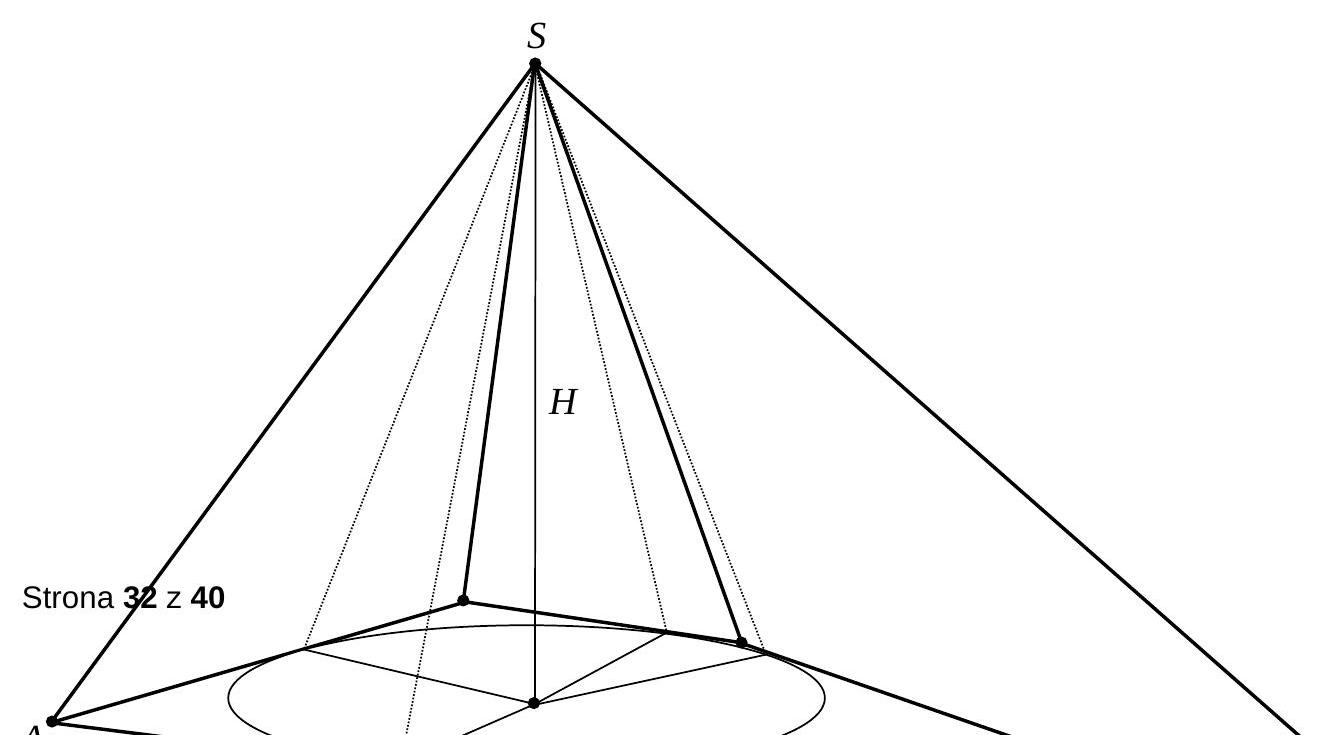
\includegraphics[max width=\textwidth]{2025_02_07_176452ab2cb6278af830g-32}
\end{center}

D

Ponieważ w tym ostrosłupie wszystkie ściany boczne nachylone są do podstawy pod tym samym kątem, więc spodek $O$ wysokości $H$ ostrosłupa jest środkiem okręgu wpisanego w wielokąt będący podstawą ostrosłupa. Niech r oznacza promień okręgu wpisanego w podstawę, $h$ - wysokość trapezu $A B C D, H$ natomiast niech oznacza wysokość ostrosłupa.\\
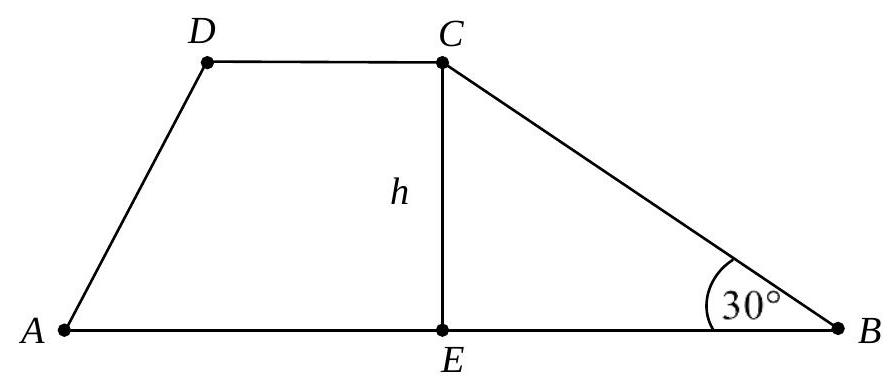
\includegraphics[max width=\textwidth, center]{2025_02_07_176452ab2cb6278af830g-33}

Ponieważ w trapez można wpisać okrąg, więc spełniony jest warunek: $|A B|+|C D|=26$. Korzystając z własności trójkąta prostokątnego $E B C$ o kątach $30^{\circ}, 60^{\circ}, 90^{\circ}$, otrzymujemy:

$$
h=|C E|=8 \text {, a stąd wynika, że } r=4 \text {. }
$$

Ponieważ $\operatorname{tg} \alpha=\frac{9}{2}$, więc $\frac{9}{2}=\frac{H}{r}$ i stąd obliczamy $H=18$.\\
Objętość tego ostrosłupa jest zatem równa

$$
V=\frac{1}{3} \cdot P_{A B C D} \cdot H=\frac{1}{3} \cdot \frac{|A B|+|C D|}{2} \cdot h \cdot H=\frac{1}{3} \cdot \frac{26}{2} \cdot 8 \cdot 18=624 .
$$

\section*{Zadanie 15. (0-7)}
\begin{center}
\begin{tabular}{|c|l|}
\hline
\multicolumn{1}{|c|}{Wymagania ogólne} & \multicolumn{1}{c|}{Wymagania szczegółowe} \\
\hline
III. Modelowanie matematyczne. & \begin{tabular}{l}
11. Rachunek różniczkowy. Zdający stosuje \\
pochodne do rozwiązywania zagadnień \\
optymalizacyjnych (R11.6). \\
\end{tabular} \\
\hline
\end{tabular}
\end{center}

\section*{Zasady oceniania I sposobu rozwiązania}
Rozwiązanie zadania składa się z trzech etapów.\\
Pierwszy etap składa się z trzech części:

\begin{itemize}
  \item przyjęcia jednego z wymiarów ekranu (długość, szerokość) za zmienną x i obliczenie drugiego wymiaru $y$ : $y=\frac{6000}{x}$.
  \item wyrażenia pola powierzchni całego ekranu z obramowaniem jako funkcji jednej zmiennej $x$ :
\end{itemize}

$$
P(x)=6 x+\frac{60000}{x}+6060
$$

\begin{itemize}
  \item wyznaczenia dziedziny funkcji $P:(2 \sqrt{1501}-2,+\infty)$.
\end{itemize}

Za poprawne wykonanie każdej z tych części zdający otrzymuje 1 punkt, o ile poprzednie kroki też były wykonane poprawnie.

Drugi etap składa się z trzech części:

\begin{itemize}
  \item wyznaczenie pochodnej funkcji $P$ lub funkcji $f(x)=6 x+\frac{60000}{x}$ określonej np. dla
\end{itemize}

$$
x>0: f^{\prime}(x)=6-\frac{60000}{x^{2}}=\frac{6 x^{2}-60000}{x^{2}}=\frac{6\left(x^{2}-10000\right)}{x^{2}} .
$$

\begin{itemize}
  \item obliczenie miejsca zerowego pochodnej funkcji $f: x=100$
  \item zbadanie znaku pochodnej funkcji $f$ : jeśli $0<x<100$, to $f^{\prime}(x)<0$ oraz jeśli $x>100$, to $f^{\prime}(x)>0$ i uzasadnienie, że dla $x=100$ funkcja $P$ przyjmuje wartość najmniejszą, na przykład: w przedziale $(2 \sqrt{1501}-2,100\rangle$ funkcja $P$ jest malejąca, w przedziale $\langle 100,+\infty)$ funkcja $P$ jest rosnąca, więc najmniejszą wartość funkcja $P$ przyjmuje dla $x=100$.
\end{itemize}

Za poprawne wykonanie każdego z tych kroków zdający otrzymuje 1 punkt, o ile poprzednie kroki też były wykonane poprawnie.

Trzeci etap polega na obliczeniu obu wymiarów ekranu: $x=100$ oraz $y=60$. Za poprawne wykonanie trzeciego etapu zdający otrzymuje 1 punkt.

\section*{Zasady oceniania II sposobu rozwiązania}
Ten sposób rozwiązania składa się z następujących czterech kroków: Rozwiązanie, w którym postęp jest niewielki, ale konieczny na drodze do pełnego rozwiązania

Jeżeli zdający przyjmie oznaczenia (na przykład x i y) na długość i szerokość ekranu, zapisze pole powierzchni całego ekranu z obramowaniem

$$
P=(x+10)(y+6)
$$

\section*{Uwaga}
Zdający, gdy przyjmie oznaczenia (na przykład x i y) na długość i szerokość ekranu, zapisze równość

$$
P=6060+6 x+10 y
$$

to otrzymuje 2 punkty.\\
Rozwiązanie, w którym jest istotny postęp 3 p.

Zdający zapisze nierówność między średnimi:

$$
\frac{6 x+10 y}{2} \geq \sqrt{6 x \cdot 10 y} .
$$

\section*{Uwaga}
Jeżeli zdający zapisze, że x i y są liczbami dodatnimi, a więc wolno skorzystać z nierówności między średnimi i zapisze nierówność między średnimi:\\
$\frac{6 x+10 y}{2} \geq \sqrt{6 x \cdot 10 y}$, to otrzymuje 4 punkty.\\
Pokonanie zasadniczych trudności zadania 5 p.\\
Zdający wykaże nierówność $P \geq 7260$.\\
Rozwiązanie prawie pełne. 6 p.

Zdający znajdzie wartości $x=100 \mathrm{~mm}, y=60 \mathrm{~mm}$.\\
Rozwiązanie pełne 7 p.\\
Zdający wyciągnie wniosek, że dla $\mathrm{x}=100 \mathrm{i} \mathrm{y}=60$ smartfon ma najmniejszą powierzchnię.

\section*{Zasady oceniania III sposobu rozwiązania}
Rozwiązanie zadania składa się z trzech etapów.\\
Pierwszy etap składa się z trzech części:

\begin{itemize}
  \item przyjęcia jednego z wymiarów całego smartfona (długość, szerokość) za zmienną x i obliczenie drugiego wymiaru całego smarfona $y$ : $y=\frac{6000}{x-10}+6$.
  \item wyrażenia pola powierzchni całego ekranu z obramowaniem jako funkcji jednej zmiennej $x$ :
\end{itemize}

$$
P(x)=x\left(\frac{6000}{x-10}+6\right)=\frac{6000 x}{x-10}+6 x .
$$

\begin{itemize}
  \item wyznaczenia dziedziny funkcji $P:(2 \sqrt{1501}+8,+\infty)$.
\end{itemize}

Za poprawne wykonanie każdego z tych etapów zdający otrzymuje 1 punkt, o ile poprzednie kroki też były wykonane poprawnie.

Drugi etap składa się z trzech części:

\begin{itemize}
  \item wyznaczenie pochodnej funkcji $P$ lub funkcji $f(x)=\frac{6000 x}{x-10}+6 x$ określonej np. dla $x>0$ :
\end{itemize}

$$
f^{\prime}(x)=\frac{6000(x-10)-6000 x}{(x-10)^{2}}+6=\frac{6\left((x-10)^{2}-10000\right)}{(x-10)^{2}}=\frac{6(x-110)(x+90)}{(x-10)^{2}} .
$$

\begin{itemize}
  \item obliczenie miejsca zerowego pochodnej funkcji $f: x=110$
  \item zbadanie znaku pochodnej funkcji $f$ : jeśli $0<x<110$, to $f^{\prime}(x)<0$ oraz jeśli $x>110$, to $f^{\prime}(x)>0$ i uzasadnienie, że dla $x=110$ funkcja $P$ przyjmuje wartość najmniejszą, na przykład: w przedziale $(2 \sqrt{1501}+8,110\rangle$ funkcja $P$ jest malejąca, w przedziale $\langle 110,+\infty)$ funkcja $P$ jest rosnąca, więc najmniejszą wartość funkcja $P$ przyjmuje dla $x=110$.
\end{itemize}

Za poprawne wykonanie każdego z tych etapów zdający otrzymuje 1 punkt, o ile poprzednie kroki też były wykonane poprawnie.

Trzeci etap polega na obliczeniu obu wymiarów ekranu: $x=100$ oraz $y=60$.\\
Za poprawne wykonanie trzeciego etapu zdający otrzymuje 1 punkt.

\section*{Uwagi}
\begin{enumerate}
  \item Jeżeli zdający rozpatruje funkcję $P$ przy założeniu, że $x+10>y+6>0$, obliczy wymiary ekranu 100 mm i 60 mm oraz obliczy wymiary smartfona 110 mm i 66 mm , i sprawdzi, że wymiary ekranu spełniają założenie $x+10>y+6$, to może otrzymać 7 punktów za całe rozwiązanie.
  \item Jeżeli zdający nie wyznaczy dziedziny funkcji $P$, ale z rozwiązania wynika, że rozważa funkcję $P$ na zbiorze, w którym co najmniej jeden z wymiarów ekranu przyjmuje wartości ujemne, to za całe rozwiązanie może otrzymać co najwyżej 5 punktów.
  \item Jeżeli zdający przyjmuje błędnie, że powierzchnia smartfona jest równa $60 \mathrm{~cm}^{2}$ i bada powierzchnię ekranu smartfona jako funkcję jednej zmiennej, to nie otrzymuje 1 punktu za 1. część l etapu rozwiązania, a w konsekwencji może otrzymać co najwyżej 6 punktów za całe rozwiązanie.
  \item Jeżeli zdający nie ujednolici jednostek, ale przeprowadzi pełne rozumowanie, to może otrzymać co najwyżej 3 punkty za całe rozwiązanie (3 punkty wyłącznie za II etap rozwiązania).
  \item Jeżeli zdający popełni błąd w zamianie $60 \mathrm{~cm}^{2}$ zapisując $600 \mathrm{~mm}^{2}$ i rozwiąże zadanie do końca, to może otrzymać co najwyżej 5 punktów.
  \item Badanie znaku pochodnej zdający może opisać w inny sposób, np. szkicując wykres funkcji, która w ten sam sposób jak pochodna zmienia znak.
  \item Za poprawne uzasadnienie, że rozważana funkcja posiada wartość najmniejszą dla wyznaczonej wartości $x$, przy której pochodna się zeruje, można uznać sytuacje, gdy zdający:\\
a) opisuje słownie lub graficznie (np. przy użyciu strzałek), monotoniczność funkcji $P$; lub\\
b) zapisuje, że dla wyznaczonej wartości $x$ funkcja $P$ ma minimum lokalne i jest to jednocześnie jej najmniejsza wartość.\\
Jeżeli zdający nie przedstawi takiego uzasadnienia, to za II etap może otrzymać co najwyżej 2 punkty.
  \item Jeżeli zdający przyjmie, że dziedziną funkcji $P$ jest przedział $(0,+\infty)$, to może otrzymać 1 punkt za 3. część II etapu, o ile otrzymane miejsce zerowe pochodnej należy do właściwej dziedziny funkcji $P$.
  \item Jeżeli zdający rozpatruje inną wielkość niż pole, np. bada obwód, to za całe rozwiązanie zadania może otrzymać co najwyżej 1 punkt za 1. część I etapu.
\end{enumerate}

\section*{Przykładowe rozwiązania}
\section*{I sposób}
Oznaczmy długości boków ekranu smartfona literami x i y ( $x>y$ ) tak jak na rysunku:\\
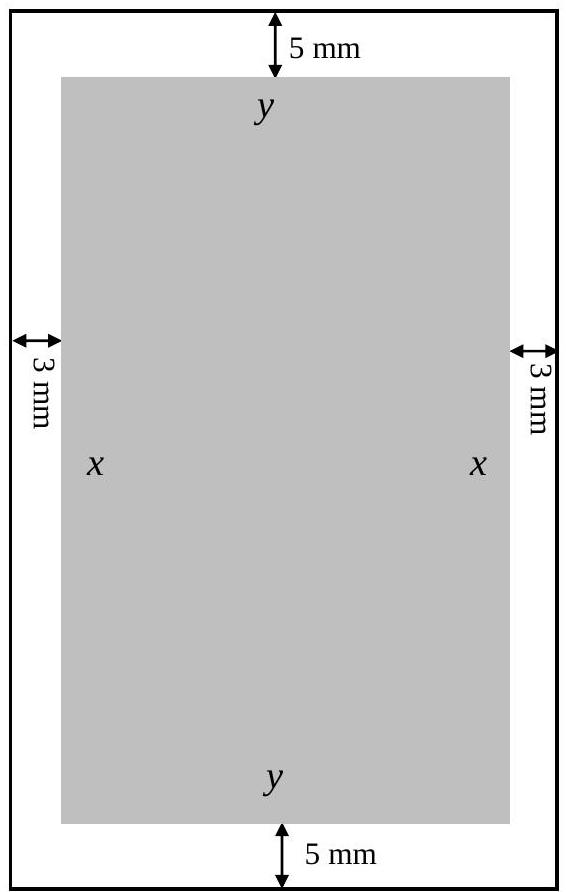
\includegraphics[max width=\textwidth, center]{2025_02_07_176452ab2cb6278af830g-37}

Wtedy powierzchnia ekranu jest równa (w mm ${ }^{2}$ ):

$$
x y=6000
$$

skąd wynika, że

$$
y=\frac{6000}{x} .
$$

Powierzchnia całego smartfona (tj. ekranu z obramowaniem) jest równa

$$
P=(x+10)(y+6)=x y+6 x+10 y+60=6000+6 x+10 y+60=6 x+\frac{60000}{x}+6060
$$

Ponieważ $x+10>y+6>0$, to $x+4>\frac{6000}{x}$. Stąd otrzymujemy kolejno:

$$
\begin{gathered}
x^{2}+4 x>6000 \\
x^{2}+4 x+4>6004 \\
(x+2)^{2}>6004 \\
|x+2|>2 \sqrt{1501} \\
x>2 \sqrt{1501}-2
\end{gathered}
$$

Otrzymaliśmy funkcję $P$ zmiennej $x$ określoną wzorem

EGZAMINACYJNA

$$
P(x)=6 x+\frac{60000}{x}+6060 \text { dla } x \in(2 \sqrt{1501}-2,+\infty) .
$$

Obliczamy pochodną funkcji $P$ :

$$
P^{\prime}(x)=6-\frac{60000}{x^{2}}=\frac{6\left(x^{2}-10000\right)}{x^{2}} \text { dla } x \in(2 \sqrt{1501}-2,+\infty) .
$$

Miejscem zerowym pochodnej funkcji $P$ jest $x=100$, gdyż\\
$2 \sqrt{1501}-2<2 \sqrt{1521}-2=2 \cdot 39-2=76<100$.\\
Ponadto $P^{\prime}(x)<0$ dla $x \in(2 \sqrt{1501}-2,100)$ oraz $P^{\prime}(x)>0$ dla $x \in(100,+\infty)$.\\
Zatem w przedziale $(2 \sqrt{1501}-2,100\rangle$ funkcja $P$ jest malejąca, a w przedziale $\langle 100,+\infty)$\\
funkcja $P$ jest rosnąca.\\
Stąd wynika, że funkcja $P$ dla $x=100$ przyjmuje najmniejszą wartość. Wtedy $y=60$.\\
Poszukiwanymi wymiarami ekranu smartfona są: $x=100 \mathrm{~mm}, y=60 \mathrm{~mm}$.

\section*{Il sposób}
Tak jak w sposobie pierwszym obliczamy w milimetrach kwadratowych powierzchnię ekranu:

$$
P=6060+6 x+10 y .
$$

Korzystamy z nierówności między średnią arytmetyczną i geometryczną:

$$
\frac{6 x+10 y}{2} \geq \sqrt{6 x \cdot 10 y}=\sqrt{60 x y}=\sqrt{60 \cdot 6000}=\sqrt{6^{2} \cdot 10000}=6 \cdot 100=600 .
$$

Stąd wynika, że

$$
P=6060+6 x+10 y \geq 6060+1200=7260 .
$$

W nierówności między średnimi równość ma miejsce wtedy i tylko wtedy, gdy wszystkie liczby występujące w tych średnich są równe.

Niech $6 x=10 y$, czyli $6 x=10 \cdot \frac{6000}{x}$.\\
Stąd otrzymujemy równanie: $x^{2}=10000$.\\
Jedynym dodatnim rozwiązaniem tego równania jest $x=100$.\\
Wtedy $y=60$. Ponieważ $P \geq 7260$ oraz dla $x=100$ i $y=60$ mamy

$$
P=110 \cdot 66=7260,
$$

więc ekran z obramowaniem ma najmniejszą powierzchnię dla $x=100$ i $y=60$.\\
Poszukiwanymi wymiarami ekranu są: $x=100 \mathrm{~mm}, y=60 \mathrm{~mm}$.

\section*{Ill sposób}
Oznaczmy długości boków całego smartfona przez x i $y(x>y)$ tak jak na rysunku:\\
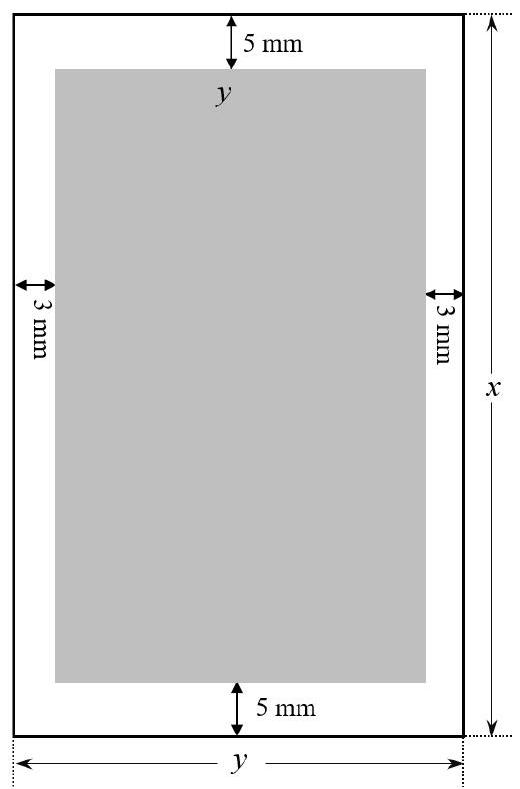
\includegraphics[max width=\textwidth, center]{2025_02_07_176452ab2cb6278af830g-39}

Wtedy powierzchnia ekranu jest równa ( $\mathrm{w} \mathrm{mm}^{2}$ ):

$$
(x-10)(y-6)=6000
$$

skąd wynika, że

$$
y=\frac{6000}{x-10}+6
$$

Powierzchnia całego smartfona (tj. ekranu z obramowaniem) jest równa

$$
P=x\left(\frac{6000}{x-10}+6\right)=\frac{6000 x}{x-10}+6 x .
$$

Ponieważ $x>y>6$ i $x>10$, to $x>\frac{6000}{x-10}+6$. Stąd otrzymujemy kolejno:

$$
\begin{gathered}
x^{2}-10 x>6000+6 x-60, \\
x^{2}-16 x+64>6004 \\
(x-8)^{2}>6004 \\
|x-8|>2 \sqrt{1501} \\
x>2 \sqrt{1501}+8
\end{gathered}
$$

Otrzymaliśmy funkcję $P$ zmiennej $x$ określoną wzorem

$$
P(x)=\frac{6000 x}{x-10}+6 x \text { dla } x \in(2 \sqrt{1501}+8,+\infty) .
$$

Obliczamy pochodną funkcji $P$ :

$$
P^{\prime}(x)=\frac{6000(x-10)-6000 x}{(x-10)^{2}}+6=\frac{6\left((x-10)^{2}-10000\right)}{(x-10)^{2}}=\frac{6(x-110)(x+90)}{(x-10)^{2}}
$$

dla $x \in(2 \sqrt{1501}+8,+\infty)$.\\
Miejscem zerowym pochodnej funkcji $P$ jest $x=110$, bo $2 \sqrt{1501}+8<2 \sqrt{1521}+8=2 \cdot 39+8=86<110$.

Ponadto $P^{\prime}(x)<0$ dla $x \in(2 \sqrt{1501}+8,110)$ oraz $P^{\prime}(x)>0$ dla $x \in(110,+\infty)$.\\
Zatem w przedziale $(2 \sqrt{1501}+8,110\rangle$ funkcja $P$ jest malejąca, a w przedziale $\langle 110,+\infty)$ funkcja $P$ jest rosnąca.\\
Stąd wynika, że funkcja $P$ dla $x=110$ przyjmuje najmniejszą wartość.\\
Wtedy $y=\frac{6000}{110-10}+6=66$.\\
Poszukiwanymi wymiarami ekranu smartfona są: $x=100 \mathrm{~mm}, y=60 \mathrm{~mm}$.


\end{document}